\section{Description of individual data sets}
\label{sec:Quality}

The CT18 global analysis includes a wide range of data from Run-1 of the LHC, in addition to the extensive collection of data used in the previous CT14 analysis with the combined HERA measurements.
Sec.~\ref{sec:data_overview} and Tables~\ref{tab:EXP_1}--\ref{tab:EXP_2}
reviewed the CT18(Z) data sets and broadly summarized the overall
quality of the fits in terms of $\chi^2/N_\mathit{pt}$ and effective Gaussian
variables $S_E$ provided for each fitted experiment.
%
A successful fit of the global data, however, requires a far more fine-grained exploration of the degree to which individual experiments are well-described.
It is important to quantitatively evaluate the agreement between data and theory with a rigorous battery of statistical measures and tests \cite{Kovarik:2019xvh}, including a
comprehensive survey of potential tensions in fitting various
experiments. We survey the landscape of experimental constraints
in Sec.~\ref{sec:QualityOverview}, concentrating
primarily on the complementary techniques of Lagrange Multiplier (LM)
scans and sensitivity calculations to elucidate the level of agreement
within the fit and remaining sources of systematic
tension. Section~\ref{sec:Qualitydata} concentrates on the theoretical
description of specific fitted experiments, while Section~\ref{sec:EW}
examines the role of NLO electroweak corrections in describing the
fitted data. 
%

Procedurally, fitting in the CT approach is done as described in App.~\ref{sec:chi2_app}. 
Firstly, we minimize the difference between data and theory by optimizing the values of the nuisance parameters $\lambda$ associated with the correlated systematic errors of each experiments. Then, we minimize $\chi^{2}$ with respect to the parameters $a$ of the functional forms of the parton distribution functions. We arrive at the best-fit  $\chi^{2}$  given by Eq.~(\ref{Chi2a0l0}) as the sum of $(D^\mathit{sh}_{i}(a_0)-T_{i}(a_0))^{2}/s_{i}^{2}$ and squares of optimal individual nuisance parameters $\overline \lambda (a_0)$. Here $T_i$ is the $i$-th theory prediction, $D^\mathit{sh}_{i}$ denotes the respective data value shifted by the optimal
systematic displacements of the nuisance parameters; $s_{i}$ is the published estimate for the total uncorrelated error.

Now, to compare data and theory, for one particular experiment, we may
plot the shifted data points $D^\mathit{sh}_{i}$ and the theory values
$T_{i}$. The error bars for the shifted data are the uncorrelated
errors $s_{i}$ only, because the correlated systematic errors are
already accounted for in the nuisance parameter values.  And there is
also a second comparison that needs to be considered: a histogram plotting
optimal nuisance parameter values $\bar \lambda_\alpha(a)$, associated
with the sources of systematic uncertainties, and usually assumed to
be sampled from a normal distribution ${\cal N}(0,1)$ with the mean
equal to 0 and standard deviation equal to 1.


\subsection{Overall agreement among experiments \label{sec:QualityOverview}}

\subsubsection{Revisiting effective Gaussian variables}
Let us first return to Fig.~\ref{fig:sn_ct18} illustrating the overall quality of individual description of experiments in the CT18 NNLO global fit based on the information collected in Tables~\ref{tab:EXP_1} and \ref{tab:EXP_2}. 
Instead of examining $\chi^2_E(N_{pt,E})/N_{pt,E}$ for individual experiments $E$, which have different probability distributions dependent on $N_{pt,E}$, we plot equivalent information in the form of a histogram of the effective Gaussian variables $S_E=\sqrt{2\chi^2_E}-\sqrt{2N_{pt,E}-1}$ listed in Tables \ref{tab:EXP_1} and \ref{tab:EXP_2} \cite{Lai:2010vv}.

If all deviations of theory from data are purely due to random
fluctuations, one would expect to recover an empirical distribution of
$S_E$ that is close to ${\cal N}(0,1)$ for any
$N_{pt,E}$. In practice, any recent global fit renders an $S_E$
distribution that is statistically incompatible with ${\cal N}(0,1)$
\cite{Kovarik:2019xvh}, indicating that too many experiments are
underfitted or overfitted compared to the textbook case.

For the CT18 NNLO fit, the observed $S_E$ distribution shown in Fig.~\ref{fig:sn_ct18} is most compatible with ${\cal N}(0.6,1.9)$. The probability that is compatible with ${\cal N}(0,1)$ is very small ($p=2.5\cdot 10^{-5}$ according to the Anderson-Darling test \cite{Kovarik:2019xvh}). In the figure, we labeled the
experiments with the largest deviations from $S_E\! =\! 0$. These are the combined HERAI+II data set on inclusive DIS \cite{Abramowicz:2015mha} with $S_E\approx 5.7$, which provides the dominant constraints on the PDFs and must be retained in the global analysis despite the quality-of-fit issues discussed in Sec.~\ref{sec:summary-HERA2}, and the CCFR measurement \cite{Seligman:1997mc} of the structure function $x_B F_3(x_B,Q)$ in charged-current DIS on iron, which has an unusually low $\chi^2/N_{pt}\approx 0.4$ for the central fit, but does constrain the PDF uncertainty for some flavors, as can be seen, {\it e.g.}, in the LM scans presented in the next section. 

We also note that the new LHC Run-1 data sets, indicated by the
light green color in Fig.~\ref{fig:sn_ct18}, have more positive than
negative $S_E$ values, indicating that their $\chi^2$ values are larger
than would be expected from random fluctuations consistent with the published experimental errors, as can be verified by consulting Table~\ref{tab:EXP_2}.

Two squares and two stars indicate the $S_E$ values for the NuTeV dimuon and CCFR dimuon data,
respectively, which we highlight for special attention given the importance of these data for probing the strangeness PDF. An analogous plot for the alternative CT18Z fit in Fig.~\ref{fig:sn_ct18z} shows increased $S_E$ values for the CCFR and NuTeV experiments, as compared to the CT18 fit, because of the conflicting pull of the ATLAS 7 TeV $W/Z$ production data. 

\begin{figure}[p]
  \hspace*{-0.6cm}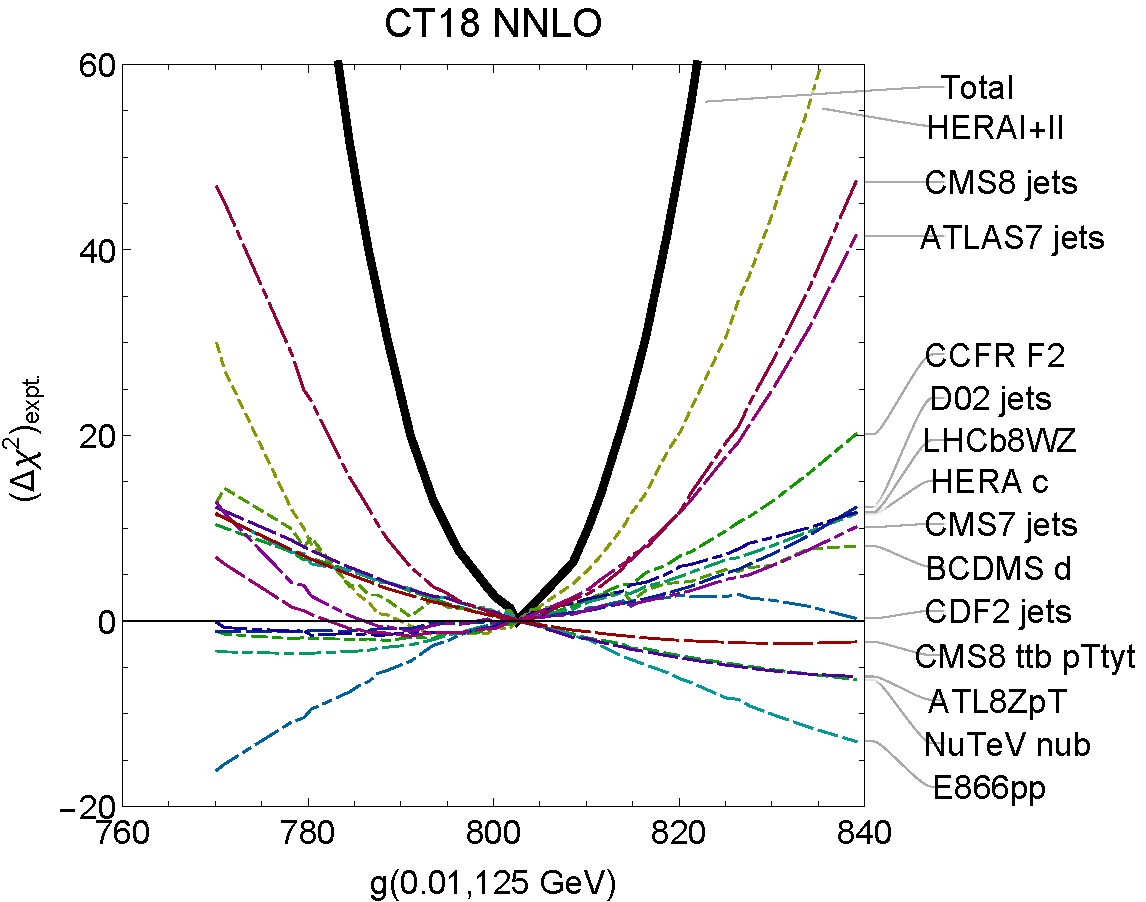
\includegraphics[width=0.45\textwidth]{./fig/gMHT_scanCT18.pdf}\quad
  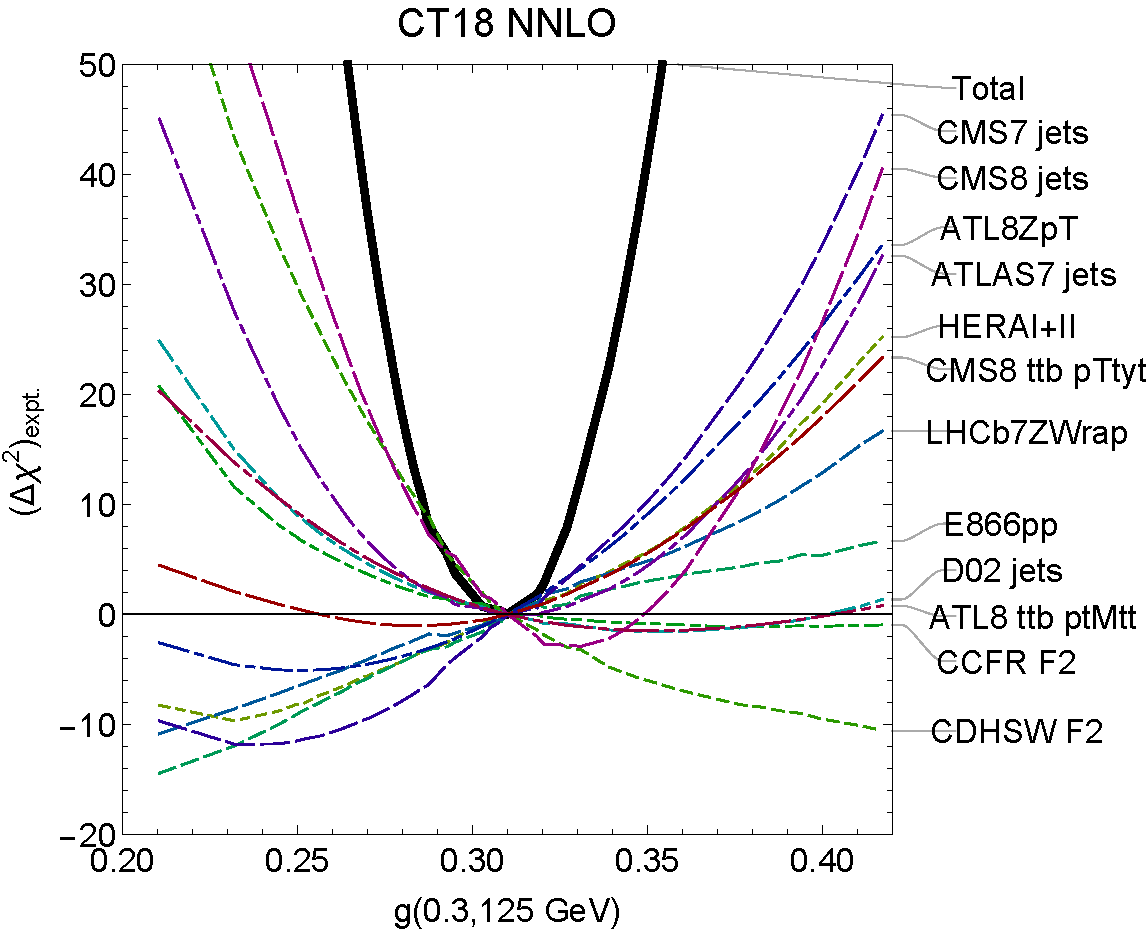
\includegraphics[width=0.43\textwidth]{./fig/gx0p3_scanCT18.pdf}
	\caption{LM scans for the gluon PDF at $Q=125$ GeV and $x=0.01$ and $0.3$, based upon the CT18 NNLO fits.
		\label{fig:LMg18}}
\end{figure}


% - - - - - - - - - - PANELS FOR u,d
\begin{figure}[p]
	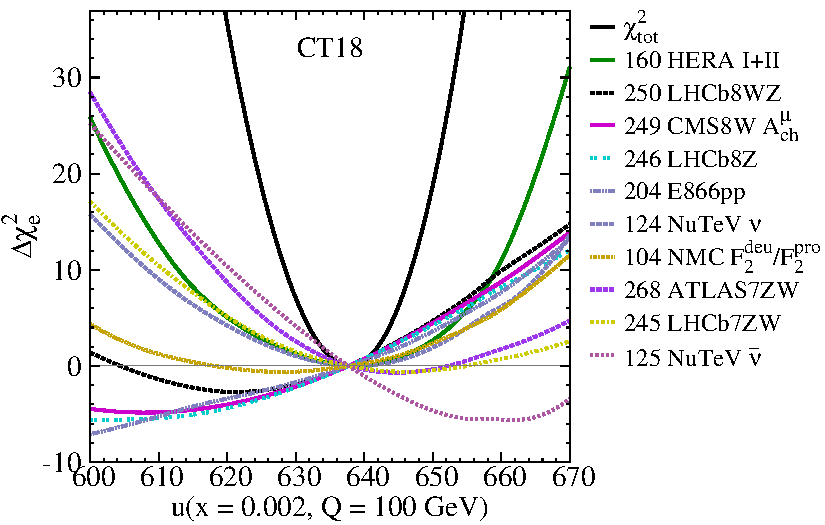
\includegraphics[width=0.49\textwidth]{./fig/pib23hTnu2E-3p0_0E00_LM27-__1_x2_00E-03_Q1_00E+02_DEchi2_re0_ect.pdf} 
	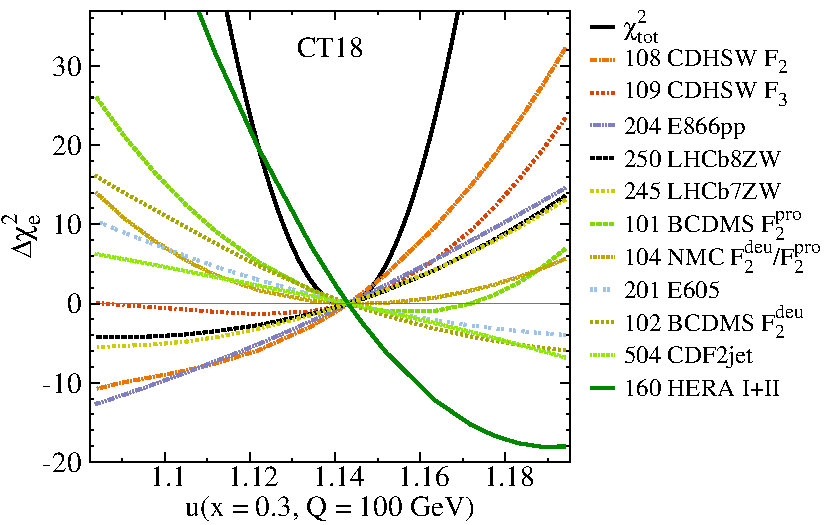
\includegraphics[width=0.49\textwidth]{./fig/pib23hTnu3E-1p1_0E1_LM27-__1_x3_00E-01_Q1_00E+02_DEchi2_re0_ect.pdf}\\
	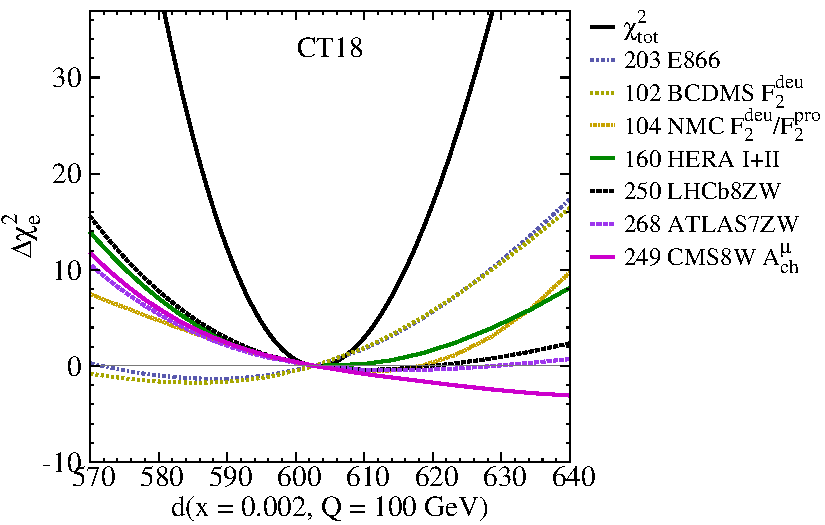
\includegraphics[width=0.49\textwidth]{./fig/LM/pib23hTnd2E-3p0_0E00_LM27-__2_x2_00E-03_Q1_00E+02_DEchi2_re0_ect.pdf}%d_lx.pdf
	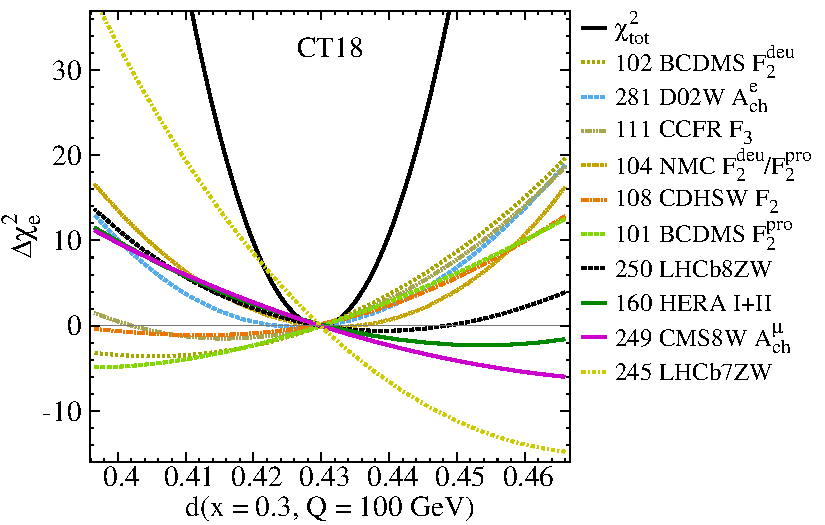
\includegraphics[width=0.49\textwidth]{./fig/LM/pib23hTnd3E-1p0_0E00_LM27-__2_x3_00E-01_Q1_00E+02_DEchi2_re0_ect.pdf}\\ %d_hx.pdf
        	\caption{LM scans for the up- and down-quark PDF at $Q=100$ GeV and $x=0.002$ and $0.3$, based upon the CT18 fits.
		\label{fig:LMud}}
\end{figure}

% - - - - - - - - - - PANELS FOR ubar, dbar, s
%
\begin{figure}[p]
	\center
	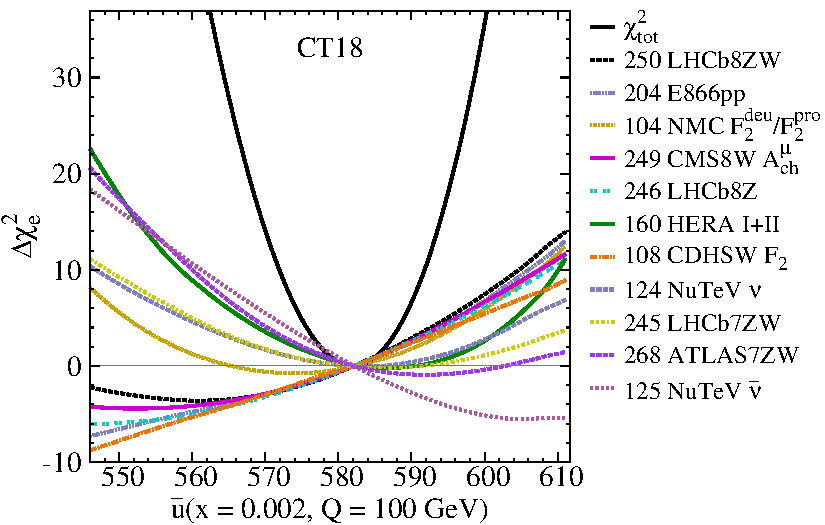
\includegraphics[width=0.49\textwidth]{./fig/LM/pib23hTnub2E-3p0_0E00_LM27-_-1_x2_00E-03_Q1_00E+02_DEchi2_re0_ect.pdf}%ub_lx.pdf
	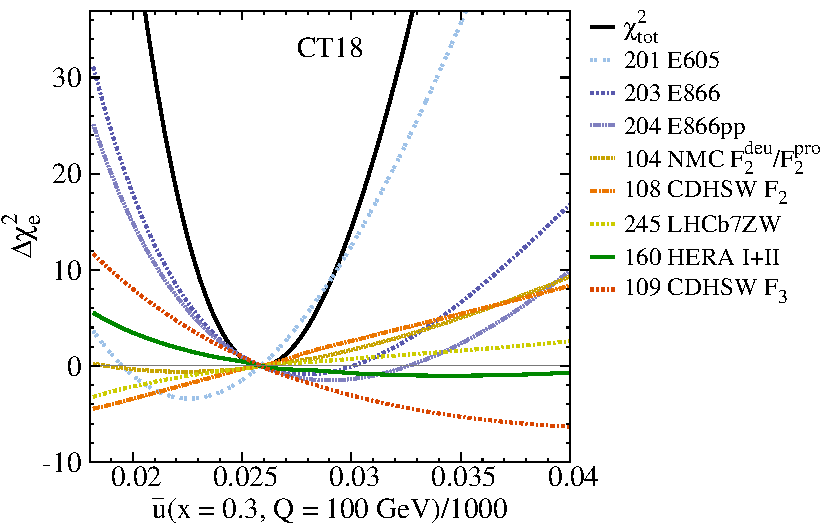
\includegraphics[width=0.49\textwidth]{./fig/LM/pib23hTnub3E-1p0_0E00_LM27-_-1_x3_00E-01_Q1_00E+02_DEchi2_re0_ect.pdf}\\ %ub_hx.pdf
	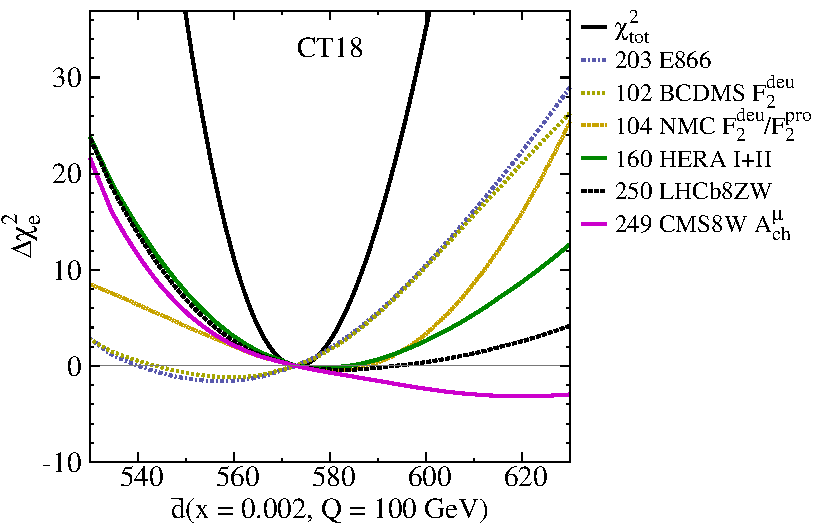
\includegraphics[width=0.49\textwidth]{./fig/LM/pib23hTndb2E-3p0_0E00_LM27-_-2_x2_00E-03_Q1_00E+02_DEchi2_re0_ect.pdf}%db_lx.pdf
	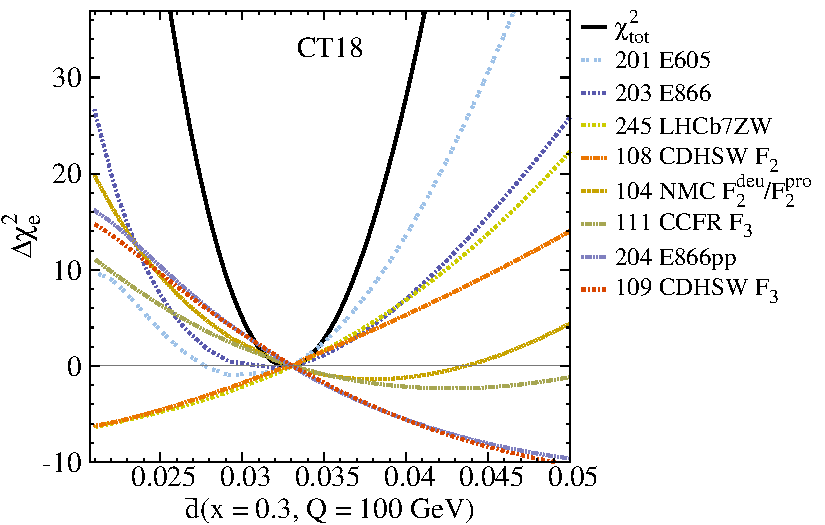
\includegraphics[width=0.49\textwidth]{./fig/LM/pib23hTndb3E-1p0_0E00_LM27-_-2_x3_00E-01_Q1_00E+02_DEchi2_re0_ect.pdf}\\ %db_hx.pdf
         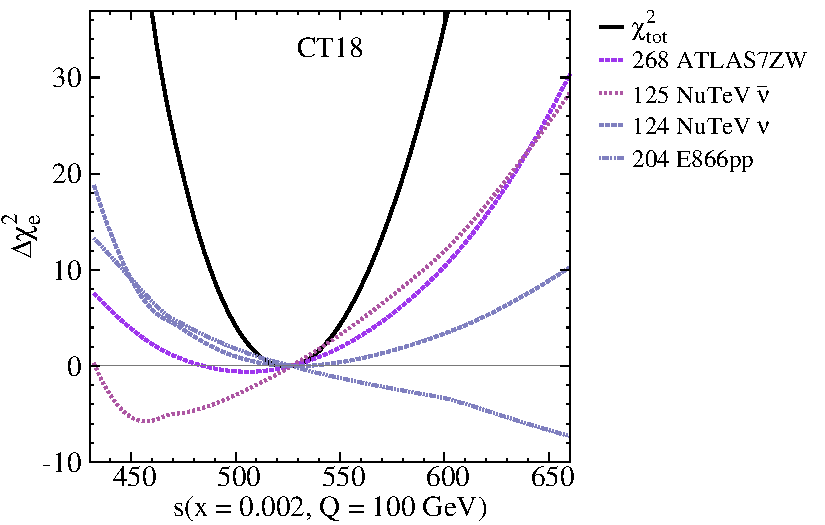
\includegraphics[width=0.49\textwidth]{./fig/LM/pib23hTns2E-3p0_0E00_LM27-__3_x2_00E-03_Q1_00E+02_DEchi2_re0_ect.pdf} %s_lx.pdf
	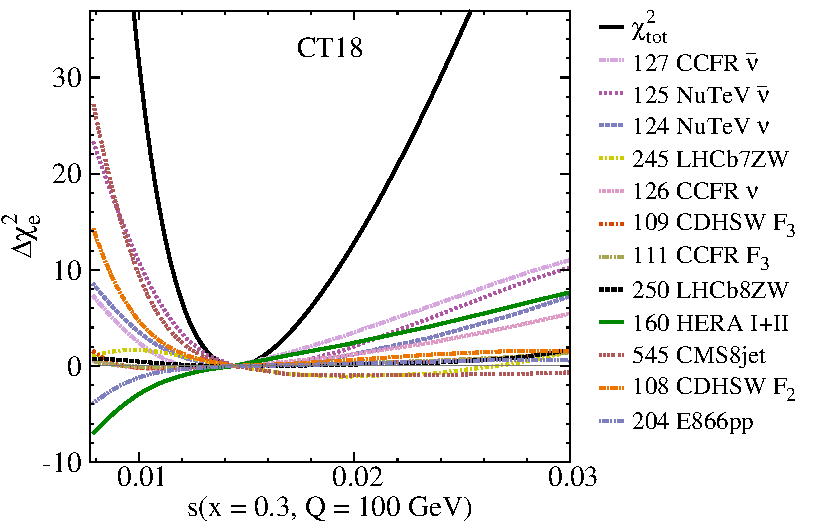
\includegraphics[width=0.49\textwidth]{./fig/LM/s_hx.pdf} %s_hx.pdf
	\caption{
		Like Fig.~\ref{fig:LMud}, here giving LM scans for the
		$\bar{u}$-, $\bar{d}$-, and $s$-quark PDFs
		in CT18.
		}
\label{fig:LMubdbs}
\end{figure}

\subsubsection{Lagrange Multiplier scans
\label{sec:LMScans}
}

The Lagrange Multiplier (LM) scan technique,
which was introduced in Ref.~\cite{Stump:2001gu}, is among the most
robust methods of assessing the level of tension in a global fit. This method involves constraining a particular fitted distribution
to hold a chosen numerical value by means of Lagrange multipliers,
while refitting the rest of the PDF parameters with this constraint
in place. A PDF at a chosen $x$ and $\Q$ can then be systematically varied away from its value preferred in an unconstrained global fit. The profile of increases in $\chi^2$ (or $S_E$) as a result of this variation can be computed for each fitted experiment, revealing the extent to which numerical alteration
of the PDFs is connected to the ability to successfully describe specific data.
%

 A collection of panels
in Figs.~\ref{fig:LMg18}--\ref{fig:LMduratios}
demonstrates $\chi^2$ profiles in LM scans
for a broad range of CT18 NNLO PDFs, typically at a high scale $\Q\!=\! 100$ GeV relevant for high-energy processes,
and for select parton fractions representative of the PDF
behavior at low $x$ ($x=0.002$ and $0.023$) and high $x$ ($x=0.1$ and
$0.3$). Among the generic features of the scans, we observe that,
while the global $\chi^2$ for all experiments is close to parabolic in
well-constrained $(x,Q)$ regions, some individual experiments may
prefer the PDF values that are quite different from the global
minimum. At the global minimum itself, the $\chi^2_E$ for such an
experiment may be elevated by up to tens of units.  

In Fig.~\ref{fig:LMg18}, for instance, we show two LM scans associated
with the gluon density, $g(x,\Q)$. In the left panel, the LM scan probes the pulls of the most sensitive measurements to the Higgs-region gluon PDF, which
contributes to Higgs boson production through the predominant $gg \to
H$ channel, especially in the neighborhood of $x = m_H /
(14\,\mathrm{TeV})\!\sim\! 0.01$ and for $\Q\!\sim\!m_H$. Evidently,
most constraints arise due to HERA inclusive DIS data as well as the
LHC jet data. 

{\color{red} Tim ---
In the right-hand plot for $x=0.3$, strong constraints spread over more data
sets, notably from high-$p_T$ $Z$ boson $p_T$ and top-quark
production. In particular, while the ATLAS 7 TeV inclusive jet data
prefer $g(0.3,125\mbox {GeV})\approx 0.3$, consistent with
the central value of the full fit, the CMS 7 TeV and 8 TeV jet
production prefer $g(0.3,125\mbox {GeV}) = 0.242^{+0.016}_{-0.020}$
and $0.327^{+0.015}_{-0.010}$ --- a $\approx 3\sigma$ difference
according to the $\Delta \chi^2=1$ criterion.
}

We notice that in some situations when a significant tension
between the experiments is revealed, as in the right-hand plot of
Fig.~\ref{fig:LMg18}, a Hessian estimate based on the
MSTW-type dynamic tolerance \cite{Martin:2009iq}
noticeably underestimates the true range of the PDF uncertainty
based on the detailed $\chi^2$ behavior
in the LM scan, as a consequence of the trade-off between the opposite
pulls on the PDF exerted by the conflicting experiments. 

%
In Fig.~\ref{fig:LMud} we show LM scans for the $u$- and $d$-quark
PDFs at $x=0.002$ and $0.3$.
%
For the low-$x$ values, constraints from  LHC $W$ and $Z$ boson data 
(from the LHCb, CMS and ATLAS collaborations) stand out
as expected, in addition to constraints from HERA and NuTeV.
%
At $x=0.3$, several fixed target experiments, e.g., CDHSW, BCDMS, and
E866 make significant contributions.
%
The situations are similar for the $d$-quark density as well as for the $d/u$ ratio shown in Fig.~\ref{fig:LMduratios}.

For the $\bar u$ and $\bar d$ antiquarks in Fig.~\ref{fig:LMubdbs}, as
well as the  $\bar d/\bar u$ ratio in Fig.~\ref{fig:LMduratios},
the LHCb data and the CMS $W$ boson charge asymmetry data play an
important role at small-$x$, as can be seen from
Fig.~\ref{fig:LMubdbs}. 
%
On the other hand, at large-$x$, the flavor separation depends on the
E605, E866 and NMC deuteron data. 

\begin{figure}[b]
\begin{center}
	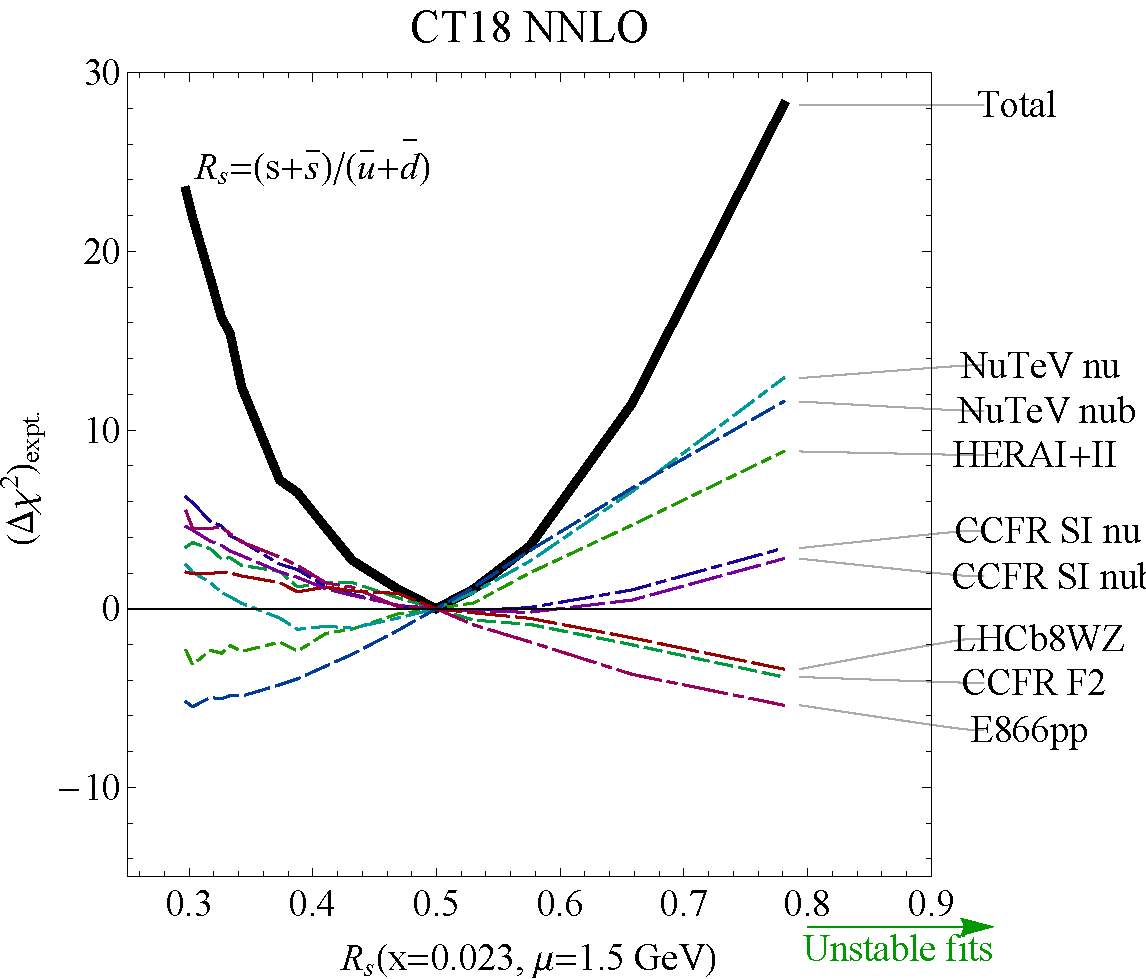
\includegraphics[width=0.48\textwidth]{./fig/Rs_scan2Tct18_1.pdf}\quad
	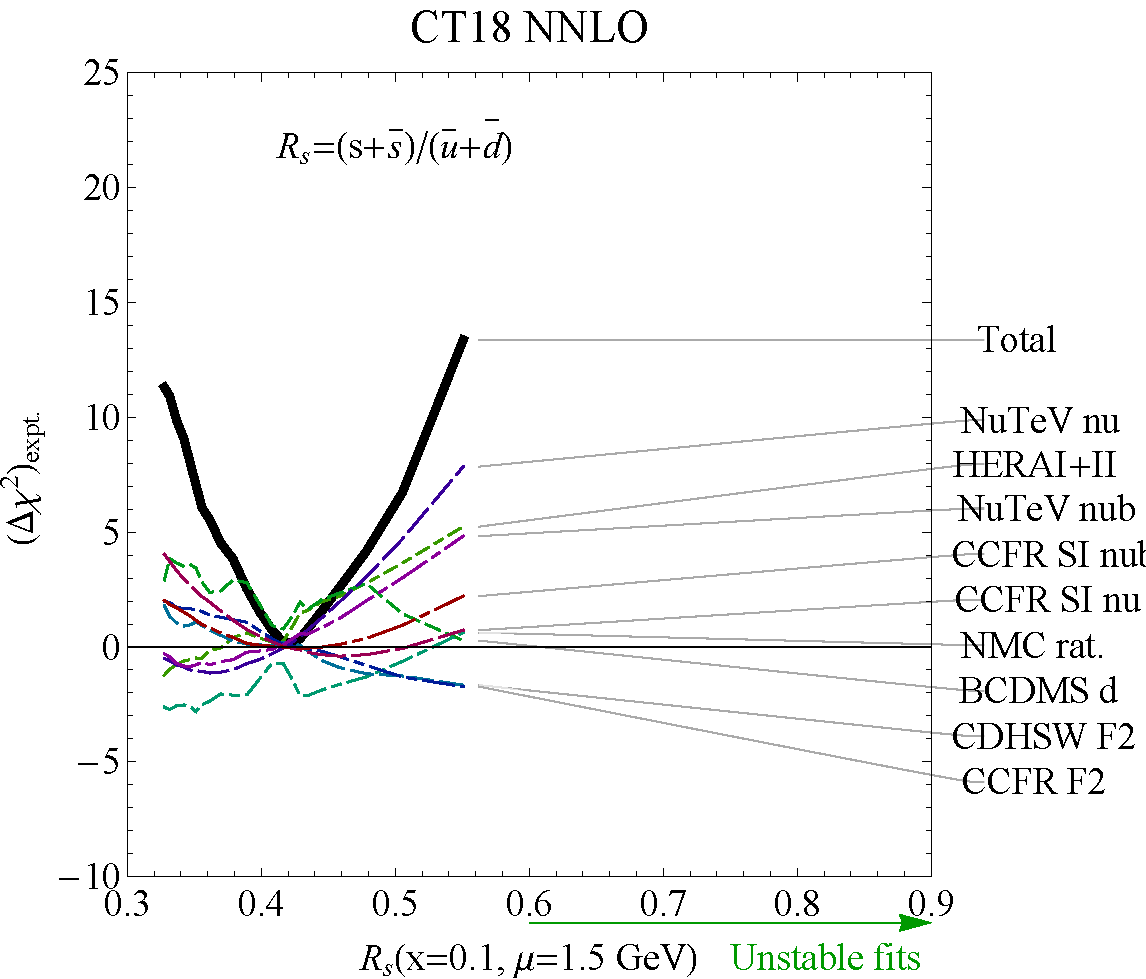
\includegraphics[width=0.48\textwidth]{./fig/Rs_scan2Tct18_2.pdf}\\
(a)\hspace{2.6in}(b)\\
	\caption{The LM scan over $R_s$ at $Q=1.5$ GeV, with $x=0.023$ and $x=0.1$ respectively, for the CT18 NNLO fit.
\label{fig:LMRs}}
\end{center}
\end{figure}

%
\begin{figure}[tb]
	\center
	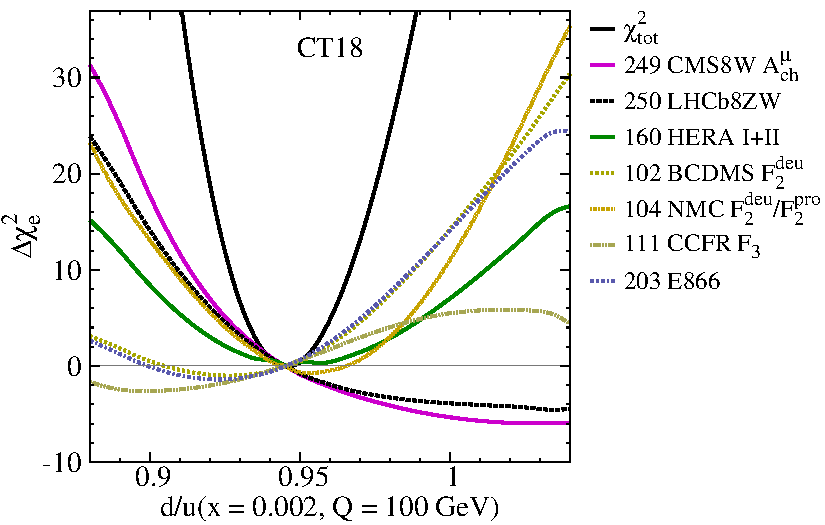
\includegraphics[width=0.49\textwidth]{./fig/LM/pib23hTndou2E-3p0_00E0_LM27-_10_x2_00E-03_Q1_00E+02_DEchi2_re0_ect.pdf} %du_lx.pdf
	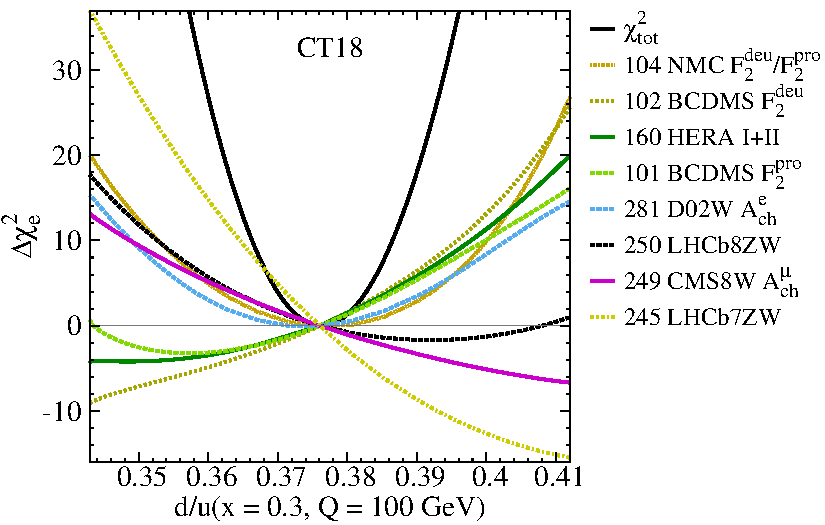
\includegraphics[width=0.49\textwidth]{./fig/LM/pib23hTndou3E-1p0_00E0_LM27-_10_x3_00E-01_Q1_00E+02_DEchi2_re0_ect.pdf}\\ %du_hx.pdf
	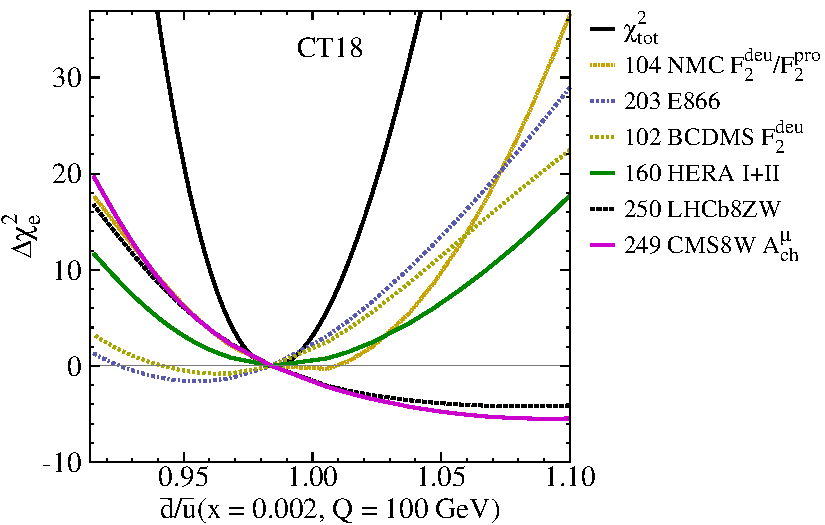
\includegraphics[width=0.49\textwidth]{./fig/LM/pib23hTndboub2E-3p0_00E0_LM27-_11_x2_00E-03_Q1_00E+02_DEchi2_re0_ect.pdf}%dbub_lx.pdf
	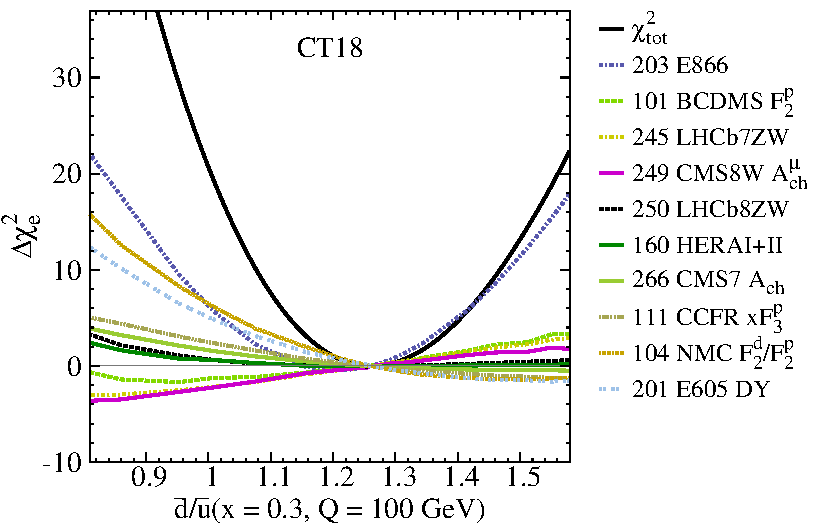
\includegraphics[width=0.5\textwidth]{./fig/LM/pjb02a20_LM25-_11_x3_00E-01_Q1_00E+02_DEchi2_re0.pdf}\\ %dbub_hx.pdf

	\caption{Like Fig.~\ref{fig:LMud}, for LM scans over the
          ratios $d/u$ and $\bar d/\bar u$. 
		}
\label{fig:LMduratios}
\end{figure}


The power of the LM method is most explicitly
demonstrated by the scans on the strange
quark PDF for CT18 in the third row of Fig.~\ref{fig:LMubdbs}, and the
strangeness ratio $R_s(x,Q)$ defined in Eq.~(\ref{eq:Rs}) and scanned at
$x=0.023$ and $x=0.3$ in Fig.~\ref{fig:LMRs}. We see from the lower
left inset of Fig.~\ref{fig:LMubdbs} at
$x=0.002$ that the CT18 data set provides no substantial direct
constraint on $s(x,Q)$ at $x < 0.01$. Rather, the behavior of $s(x,Q)$ is
weakly constrained by the low-luminosity ATLAS 7 TeV $W$ and $Z$ data
(Exp.~ID=268), as well as by the low-$x$ extrapolation of the constraints by
the NuTeV and CCFR dimuon data probing $x$ above $0.01$.

At $x=0.01\!-\!0.1$, the $R_s$ ratios in Fig.~\ref{fig:LMRs} indicate the
dominance of constraints from NuTeV and CCFR dimuon production,
together with HERA inclusive DIS, with weaker constraints from
LHCb $W/Z$ production
and the fixed-target experiments BCDMS, CDHSW, E866, and NMC. Here, the scans
reveal a salient feature, that the fits using the CT18
strangeness parametrization become unstable when $R_s(x,Q)$ is forced
to be close to 1 at $x > 0.01$. For such increased $R_s$ values, the
$\chi^2$ values fluctuate, or the fits fail to converge. Somewhat
larger values of $R_s$ are tolerated at $x < 0.01$. 

Finally, going back to $s(x,Q)$ at $x=0.3$ in the lower right inset of
Fig.~\ref{fig:LMubdbs}, the very large-$x$ behavior is again
determined by the extrapolation of the strangeness PDF from lower $x$,
where it is constrained by the combination of the experiments listed
in the figure. 

We see from this Section that the advantage of the Lagrange Multiplier approach lies in its systematic, robust nature, as well as its ability to reveal tensions or
instabilities that may be missed by the other techniques.
On the other hand, this calculation requires repeated refits
of the PDFs for many values of the LM parameter(s) ---
a limitation that makes the LM scans computationally expensive.

% ~ ~ ~ ~ ~ ~ ~ ~ ~ ~ ~ ~ ~ ~ ~ ~ ~ ~ ~ ~ ~ ~ ~ ~ ~ ~ ~ ~ ~ ~ ~ ~ ~ ~ ~ ~ ~ ~ ~ ~ ~ ~ ~ ~ ~ ~ ~ ~ ~ ~
%
\subsubsection{The PDF sensitivity analysis
\label{sec:L2}
}
%
A technique complementary to the LM scans explored in Sec.~\ref{sec:LMScans}
is the calculation of the {\it $L_2$ sensitivity}. The $L_2$ sensitivity was
first introduced in Ref.~\cite{Hobbs:2019gob} for the purpose of analyzing
the interplay among the pulls of the CT18(Z) data upon the fitted PDFs.
Here we will review its essential definition. A closely related
implementation, based on the $L_1$ sensitivity detailed
in \cite{Wang:2018heo} and realized in the \texttt{PDFSense} program,
will be used at the end of this Section to rank the experiments of the
CT18 data set according to the sensitivity to various combinations of PDFs.
  
%
%
While the LM scans offer the most robust approach for exploring
possible tensions among fitted data sets in a given analysis, they are
very computationally costly to evaluate and 
done for specific choices of $x$ and $Q$.
As we explain here, the $L_2$ sensitivity can be rapidly
computed and provides a strong approximation to the $\Delta \chi^2$
trends in
a given global analysis. Moreover, the $L_2$ sensitivity can be
readily calculated across a wide range of $x$, allowing the $\Delta \chi^2$
variations shown in the LM scans to be visualized and interpreted
for multiple $x$ at once. We stress that the qualitative conclusions
revealed by consideration of the $L_2$ sensitivities, discussed and
presented below, are consistent with the picture based on the LM
scans themselves.
Although the $L_2$ sensitivities may not always provide the same
numerical ordering as the LM scans for the subdominant experiments,
they offer complementary information over broader reaches of $x$
that are not completely captured by the LM scans.


We work in the Hessian formalism \cite{Pumplin:2002vw,Nadolsky:2008zw,Pumplin:2001ct} and compute the $L_2$ sensitivity $S_{f, L2}(E)$ for each experiment, $E$, as
%
%
\begin{equation}
S_{f, L2}(E) = \vec{\nabla} \chi^2_E \cdot \frac{ \vec{\nabla} f } { |\vec{\nabla} f| }
             = \Delta \chi^2_E\, \cos \varphi (f, \chi^2_E)\ ,
\label{eq:L2}
\end{equation}
%
%
which yields the variation of the log-likelihood function $\chi^2_E$ due to a unit-length
displacement of the fitted PDF parameters away from the global minimum $\vec{a}_0$ of
$\chi^2(\vec{a})$  in the direction of $\vec{\nabla}f$. 
The PDF parameters $\vec a$ are normalized so that a unit displacement
from the best fit in any direction corresponds to the default
confidence level of the Hessian error set (90\% for CT18,
on average corresponding to slightly less than
$\Delta\chi^2_{\textrm{tot}}=100$ in a given direction.)

This displacement increases the
PDF $f(x,Q)$ by its Hessian PDF error $\Delta f$, and, {\color{red} (TIM) to the extent its
PDF variation is correlated with that of $\chi^2_E$ through the correlation angle}
%
\begin{equation}
	\varphi(f, \chi^2_E) = \cos^{-1} \left( \frac{\vec{\nabla} f}{|\vec{\nabla} f |} \cdot \frac{\vec{\nabla} \chi^2_E}{|\vec{\nabla} \chi^2_E |} \right)\ ,
\end{equation}
%
it changes $\chi^2_E$ by $\Delta \chi^2_E (\hat{a}_f) = \Delta \chi^2_E\, \cos \varphi (f, \chi^2_E) = S_{f, L2}(E)$.
%
%
The $L_2$ sensitivity, $S_{f, L2}(E)$, therefore quantifies the impact variations of PDFs
at fixed $x$ and $Q$ have upon the description of fitted data sets.  Plotting $S_{f, L2}(E)$
against $x$ yields useful information regarding the pulls of the CT18(Z) data sets 
upon PDFs (and PDF combinations) fitted in the global analysis. This also permits
the rapid visualization of possible tensions within the global fit, since
the PDF variation of some parton densities of given flavor are correlated with the
variation of $\chi^2_E$ ({\it i.e.}, $S_{f, L2}(E) > 0$), while others are
anti-correlated ($S_{f, L2}(E) < 0$), at the same values of $(x, Q)$.

The terms on the right-hand side of Eq.~(\ref{eq:L2}) for $S_{f,L2}$
are computed as
\begin{equation}
\Delta X=\left\vert \vec{\nabla}X\right\vert
=\frac{1}{2}\sqrt{\sum_{i=1}^{N_{\textrm{eig}}}\left(X_{i}^{(+)}-X_{i}^{(-)}\right)^{2}},\label{masterDX}
\end{equation}
and
\begin{equation}
\cos\varphi=\frac{\vec{\nabla}X\cdot\vec{\nabla}Y}{\Delta X\Delta
  Y}=\frac{1}{4\Delta X\,\Delta
  Y}\sum_{i=1}^{N_{\textrm{eig}}}\left(X_{i}^{(+)}-X_{i}^{(-)}\right)\left(Y_{i}^{(+)}-Y_{i}^{(-)}\right),\label{cosphi}
\end{equation}
from the values $X_{i}^{(+)}$ and $X_{i}^{(-)}$ that a quantity
$X$ takes for the parameter displacements
along the ($\pm$) direction of the $i$-th
eigenvector. With these symmetric master formulas, the sum of
$S_{f,L2}(E)$ over all experiments $E$ should be within a
few tens from zero, since the tolerance boundary for the total $\chi^2$ is close to being spherically
symmetric. The $S_{f,L2}(E)$ variables for individual experiments tend to
cancel among themselves to this accuracy; the order of magnitude 
of $S_{f,L2}(E)$ can be also interpreted as a measure  of tension of
$E$ against the rest of the experiments. 

The $L_2$ sensitivity can be computed for individual data point
residuals or optimal nuisance parameters, {i.e.}, for parts of
Eq.~(\ref{Chi2a0l0}). A related, similarly informative,
definition of sensitivity \cite{Wang:2018heo} is computed using the absolute values
of residuals, $|r_i|$, rather than their squares $r_i^2$ (using the
$L_1$ norm instead of the $L_2$ norm). 

\begin{figure}[!htbp]
	\begin{center}
		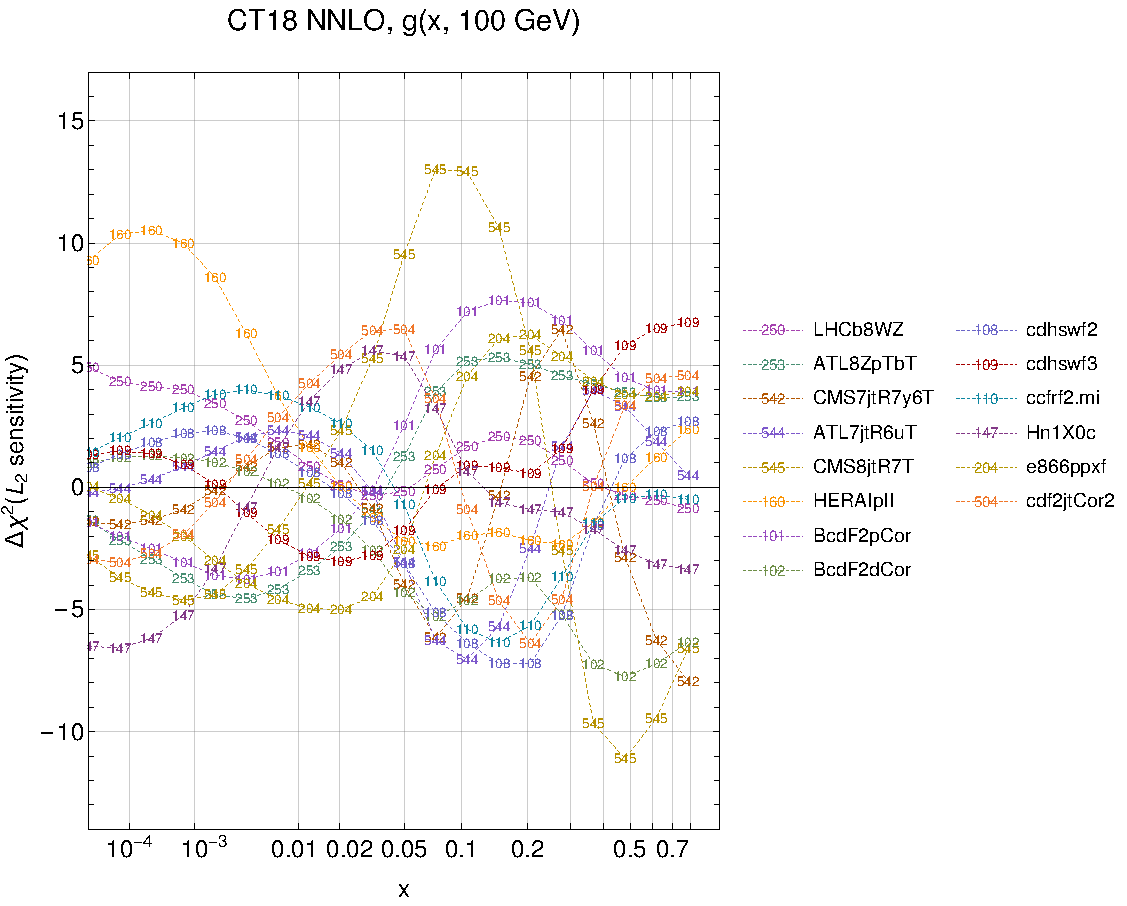
\includegraphics[width=0.85\textwidth]{./fig/Sens/ifl0_ct18nn_L2_q100_Sf_1.pdf}
	\end{center}
	\vspace{-2ex}
	\caption{
		The $x$-dependent $L_2$ sensitivity of the CT18 data sets with strongest
		pull upon the gluon PDF, $g(x,Q\!=\!100\,\mathrm{GeV})$. A number of tensions
		among the leading data sets are revealed by examining those regions of $x$
		where $S_{f, L2}(E)$ peaks for certain experiments in the `positive
		direction' while $S_{f, L2}(E)$ is sharply negative for others. For
		instance, the very high-$x$ region, $x\! \gtrsim\! 0.3$, is marked by
		strong competing pulls between the CMS 8 TeV jet data (Exp.~ID=545) --- which
		favors variation of $g(x\! \sim\! 0.3, Q\! =\! 100\,\mathrm{GeV})$ in the same
		direction as the BCDMS $F^d_2$ data (Exp.~ID=102) --- and the CMS 7 TeV jet data (Exp.~ID=542).
		The CMS 7 TeV jet data, on the other hand, have a pull on the gluon that
		aligns with that of the ATLAS 8 TeV $Z$ $p_T$ data (Exp.~ID=253) in this region. Similar
		tensions are apparent for $x\! \sim\! 0.1$ where the pull of the CMS 8 TeV
		jet data (Exp.~ID=545) is especially large, as well as in the $x\! \sim\! 0.01$
		Higgs region.
	}
\label{fig:L2glu}
\end{figure}

An extensive collection of the $L_2$
sensitivity plots for CT18(Z) PDFs and PDF ratios, reflecting the
interplay and competing pulls among the CT18 data sets, 
can be viewed at \cite{CT18L2Sensitivity}. Analogous calculations are shown for the
alternative CT18Z fit in Sec.~\ref{sec:LMCT18Z}.

In Fig.~\ref{fig:L2glu}, we show the $L_2$ sensitivity of the CT18 data
on the gluon PDF at fixed $Q\! =\! 100$ GeV, plotting curves for those
experiments that satisfy $|S_{f, L2}(E)| \ge 4$ for any value of $x$.
This criterion generally identifies the leading $\sim\! 5-10$ experiments with
strongest pull on the PDF in the kinematical region under consideration.
By its proximity to the Higgs mass scale, $Q\!=\!100$ GeV,
Fig.~\ref{fig:L2glu} highlights the opposing pulls of a number of CT18
data sets relevant for the 14 TeV Higgs boson production cross section,
$\sigma_H (14\,\mathrm{TeV})$, and is the $L_2$-based counterpart
to Fig.~\ref{fig:LMg18} (left). Of the newly-fitted LHC Run-1 data 
in CT18, the 8 TeV $Z$ $p_T$ ATLAS data
(Exp.~ID=253) show the strongest overall pull in the immediate vicinity of $x=0.01$, $S_{g, L2}(E)\, \sim\, -(4\!-\!5)$, {\color{red} (TIM) approaching the pull of the E866 $pp$
absolute cross section data (Exp.~ID=204) in the same neighborhood.
Meanwhile, the} corresponding pulls of the inclusive jet-production data are still larger
at slightly higher $x\! \sim\! 0.05-0.1$.  The effect of the Run-1 data is partially overshadowed immediately near $x\! =\! 0.01$ by the pull of the combined
HERA I+II data (Exp.~ID=160), for which we find $S_{g, L2}(\mathrm{Exp.~ID=160}) \gtrsim 5$
for $Q\! =\! 100$ GeV.  For $x\!\lesssim\! 0.1$, the CMS 8 TeV jet data (Exp.~ID=545)
have a very strong pull of $S_{g, L2}(E)\! \approx\! +13$, in contrast to the ATLAS and CMS 7 TeV jet data
(Exp.~ID=544, 542), which have somewhat weaker pulls in the opposing direction. These observations are consistent
with our findings based on the LM scans appearing in Sec.~\ref{sec:LMScans}, as typified by
Fig.~\ref{fig:LMg18} (left panel), wherein we identified the same experiments as imposing
the most stringent constraints upon $g(x\!=\!0.01, Q\!=\!m_H)$.

\begin{figure}[p]
\center
  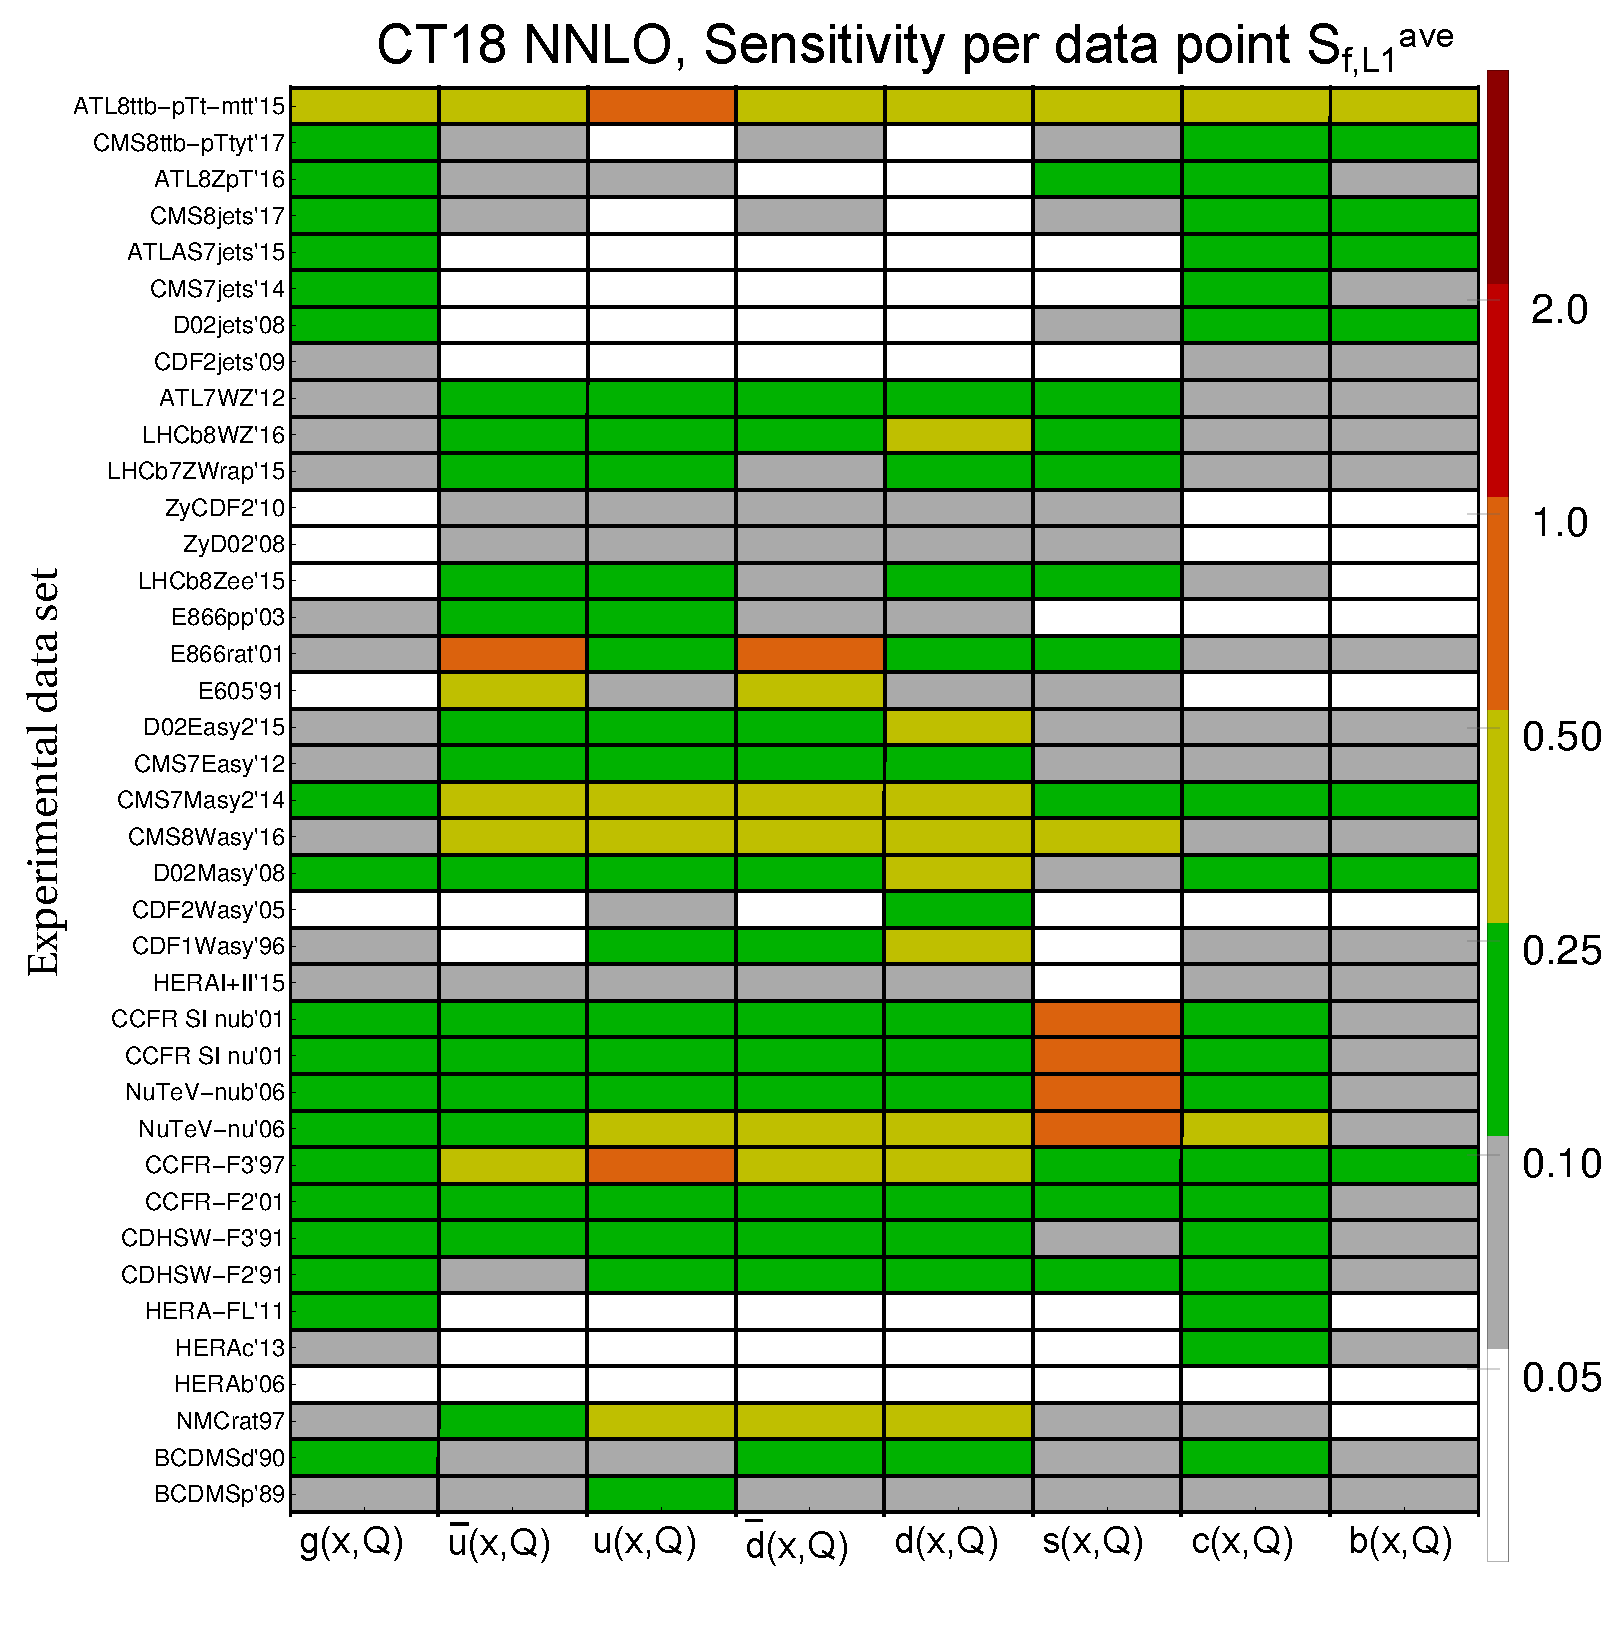
\includegraphics[width=0.59 \textwidth]{./fig/ave_S_bycolor_ct18nn.pdf}\\ 
  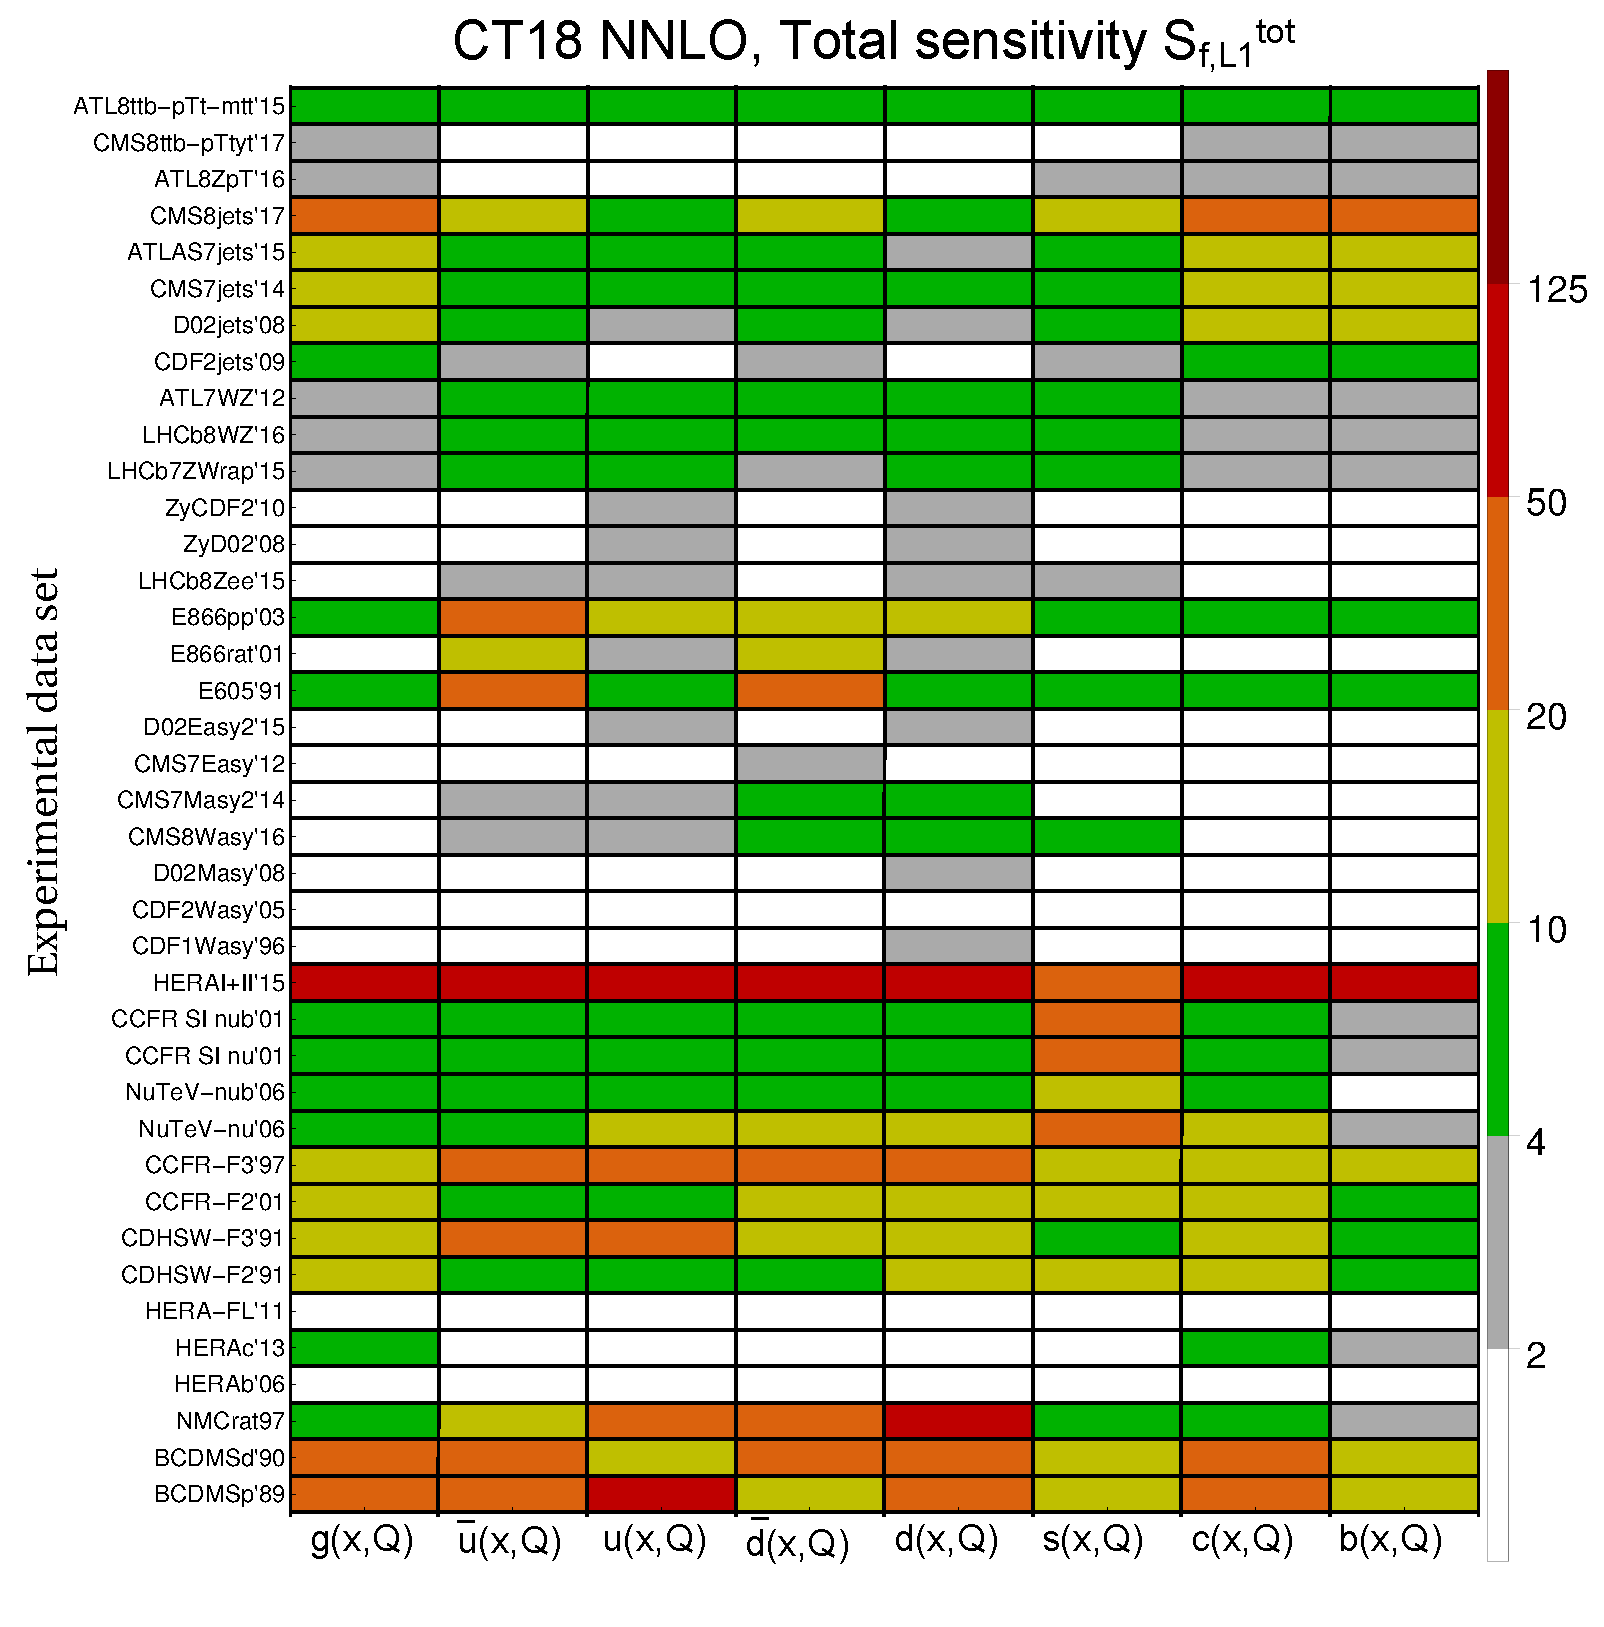
\includegraphics[width=0.59\textwidth]{./fig/total_S_bycolor_ct18nn.pdf}
        	\caption{$L_1$ sensitivities of experimental data
                  sets to PDF flavors in the CT18 NNLO analysis,
                  computed according to the methodology in
                  Ref.~\cite{Wang:2018heo}. The color of the cells
                  in the upper (lower) inset, 
                  chosen according to the palettes on the right,
                  indicates the point-average
                  (cumulative) sensitivity of the experimental set
                  on the vertical axis to the PDF flavor
                  on the horizontal axis. 
		\label{fig:CT18quilts}}
\end{figure}


The pulls and tensions on the behavior of the high-$x$ gluon
distribution can be similarly understood by examining
Fig.~\ref{fig:L2glu} at $x\! \gtrsim\! 0.3$, which is also marked by a
number of very strong competing pulls. Among the more striking of
these is the opposing alignment of the CMS 7 and 8 TeV jet-production data. 

We conclude this section by presenting 
Fig.~\ref{fig:CT18quilts} with the ranking plots of $L_1$
sensitivities computed by the \texttt{PDFSense} code
according to the approach in Ref.~\cite{Wang:2018heo}.
In that article, we presented tables that
rank the experiments in the \CTHERAII~NNLO analysis either according to
their total sensitivity to the PDFs, $f(x_i,Q_i)$, computed as
\begin{equation}
S_{f,L1}^{\textrm{tot}}(E)\equiv\sum_{i=1}^{N_{pt,E}} \left|S_{f,L1}(i)\right|,
\label{SfL1tot}
\end{equation}
or according to the average sensitivity per data point,
\begin{equation}
S_{f,L1}^{\textrm{ave}}(E)\equiv S_{f,L1}^{\textrm{tot}}(E)/N_{pt,E}.
\label{SfL1ave}
\end{equation}
These quantities respectively
estimate either the total sensitivity of the experiment $E$
to the PDF, $f(x_i,Q_i)$, at the typical $(x_i, Q_i)$ probed by data
points $i=1,..,N_{pt,E}$, and summed over all $N_{pt,E}$ points; or the
averaged sensitivity for a single data point in this experiment.
The two sensitivities allow
informative side-by-side comparison of the strengths of
constraints from individual experiments, once again estimated in the
Hessian approximation.  

In Fig.~\ref{fig:CT18quilts}, we present a graphical visualization of the ranking tables from
Ref.~\cite{Wang:2018heo}, now recomputed for the CT18 NNLO fit, and, for the most part, leading to similar conclusions as obtained for
\CTHERAII~NNLO.  The upper and lower panels of Fig.~\ref{fig:CT18quilts} correspond to the point-averaged and total
sensitivities, respectively, as discussed above. At right are placed palettes
relating the colors to the magnitudes of $S_{f,L1}(E)$.
The cells that vary from yellow to orange to red
indicate experiments (listed on the left)
with increasingly strong sensitivities to the PDFs,
$f(x,\mu)$, given at the bottom.
White or grey cells indicate experiments
with minimal sensitivity to $f(x,\mu)$.

We observe that, while the HERA I+II, BCDMS, and NMC data sets have
relatively low per-point sensitivity as seen in the upper panel,
when aggregated over their large number of points, the experiments have
very large total sensitivities to all PDF flavors
seen in the lower inset. The specialized fixed-target
measurements, such as CCFR, NuTeV, E605, and E866, are most sensitive
to certain flavors, such as $s$, $\bar u$, and $\bar d$, as expected. 

Several LHC experiments, on the other hand, have strong per-point sensitivities,
especially $t\bar t$ and high-$p_T$ $Z$ production, as
well as CMS $W$-charge asymmetries at 7 and 8 TeV (see the upper
inset). The total sensitivities of these experiments in the lower inset
are still quite low because of their small numbers of data points
($N_{pt,E}\approx 10-20$). On the other hand, the inclusive
jet production data sets
by ATLAS and CMS at 7 TeV, and especially by CMS at 8 TeV,
despite their modest sensitivities per data point, show the highest
total sensitivities among all LHC experiments because of their large
numbers of data points and extended kinematic coverage.

In aggregate, while the bulk of the sensitivity in the CT18 fit
still arises from HERA and fixed-target data, the LHC
experiments could already reduce some PDF uncertainties, given their
sizable per-point sensitivities. These uncertainty reductions have not
yet been fully realized in part due to the tensions among some LHC experiments
expounded upon earlier in the paper. 

% ~ ~ ~ ~ ~ ~ ~ ~ ~ ~ ~ ~ 
%
\subsection{Description of data sets fitted in CT18}
\label{sec:Qualitydata}
%
%
In this subsection, we illustrate the ability of CT18 to describe the individual
experiments included in this analysis, with particular attention paid to the
newly included LHC Run-1 data. We organize this discussion according to the specific
physical process.


% ~ ~ ~ ~ ~ ~ ~ ~ ~ ~ ~ ~ 
%
%
% W/Z/DY
\begin{figure}[tb]
	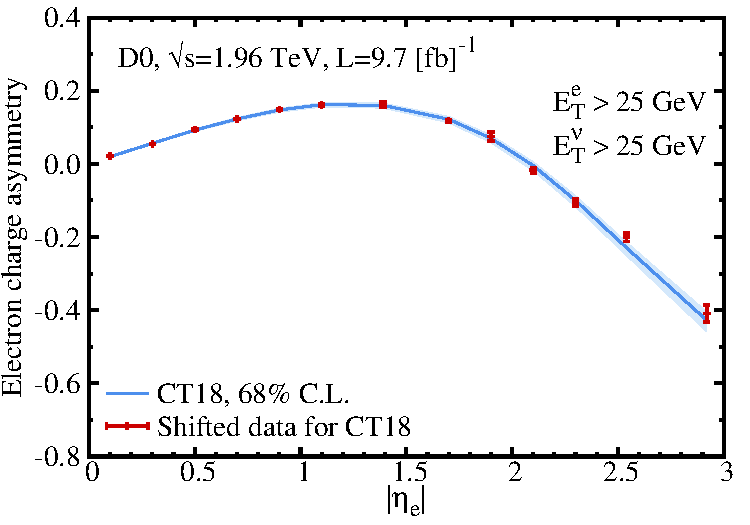
\includegraphics[width=0.49\textwidth]{./fig/data_281_CT18_abs_ect.pdf}
	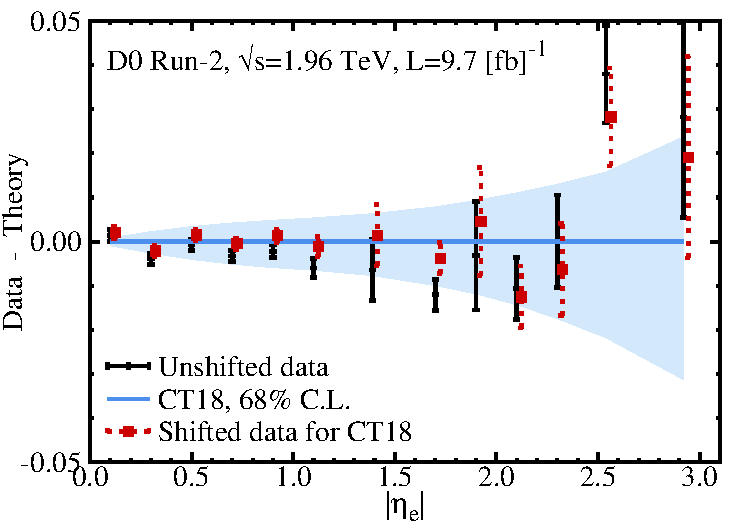
\includegraphics[width=0.49\textwidth]{./fig/data_281_CT18_DoT_v2_ect.pdf}
	\caption{
	A comparison of the CT18 theory with the D0 Run II electron charge-asymmetry data (Exp.~ID=281). Since the asymmetry crosses zero in the shown range, the right panel shows the {\it difference}, $\mathrm{Data}\!-\!\mathrm{Theory}$, rather than the {\it ratio}, $\mathrm{Data}/\mathrm{Theory}$, as done elsewhere in this section.
	}
\label{fig:281}
\end{figure}

\subsubsection{Vector boson production data}
\label{sec:QualityDYdata}
%
{\bf Tevatron charge asymmetry.}
%
CT18 PDFs show a good overall agreement with the vector boson production data from fixed-target and Tevatron experiments. In particular, the high-luminosity charge asymmetry data set 281 from D0 Run-2 \cite{D0:2014kma}, used in our analysis since CT14 \cite{Dulat:2015mca} and sensitive to $d(x)/u(x)$ at $x>0.1$, is well described.\footnote{According to the $L_2$ sensitivity \cite{CT18L2Sensitivity}, the NMC DIS data 104 and the charge asymmetry data set 281 prefer to have a softer $d(x)/u(x)$ at large $x$ by about (15) 5 units of $\chi^2_E$, compared to the full data, in contrast to the LHCb 7 TeV W rapidity (245) and E866 $pp$ Drell-Yan (204) data sets that prefer a harder $d/u$ in the same $x$ region.}

%
Fig.~\ref{fig:281} shows a data versus theory comparison for the electron charge asymmetry as a function of the absolute value of the electron pseudorapidity.
Shifted data are represented by red points, while unshifted data are black. 
The absolute charge asymmetry is illustrated in the left inset of Fig.~\ref{fig:281}, while in the right one we show the 
$\mathrm{Data}\!-\!\mathrm{Theory}$ difference where the error bars represent the total uncorrelated uncertainty for both the shifted and unshifted data, as we show consistently
throughout this section.
The theoretical predictions are computed using the code \texttt{ResBos} at approximate NNLO + NNLL in QCD. 
The blue band represents the CT18 PDF uncertainty evaluated using the Hessian symmetric errors at 
the 68\% C.L. We see that the data are described well by the CT18 predictions, with the 
exception of one high pseudorapidity bin ($|\eta_{e}|\sim2.6$), in which we observe a mild disagreement. 


%LHCb
\begin{figure}[tbp]
	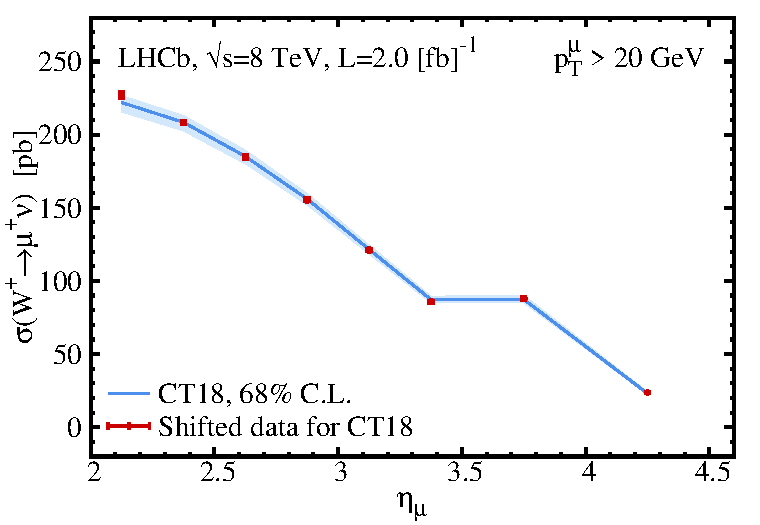
\includegraphics[width=0.49\textwidth]{./fig/data_250_CT18__1_abs_ect.pdf}
	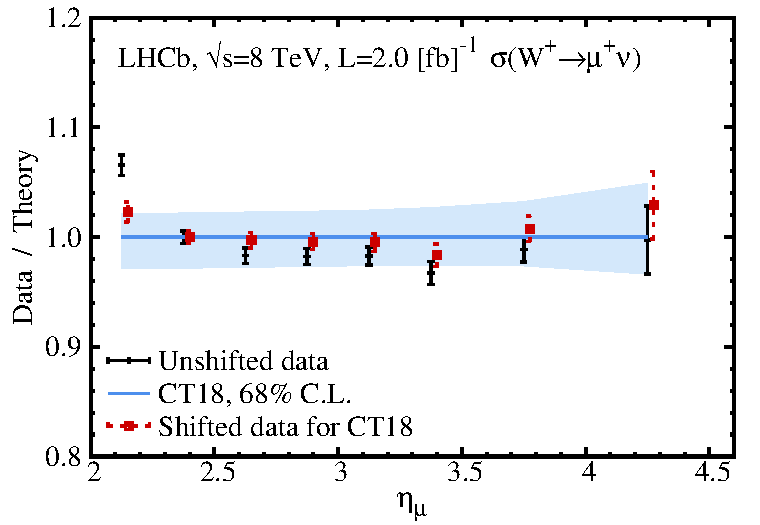
\includegraphics[width=0.49\textwidth]{./fig/data_250_CT18__1_DoT_ect.pdf}
	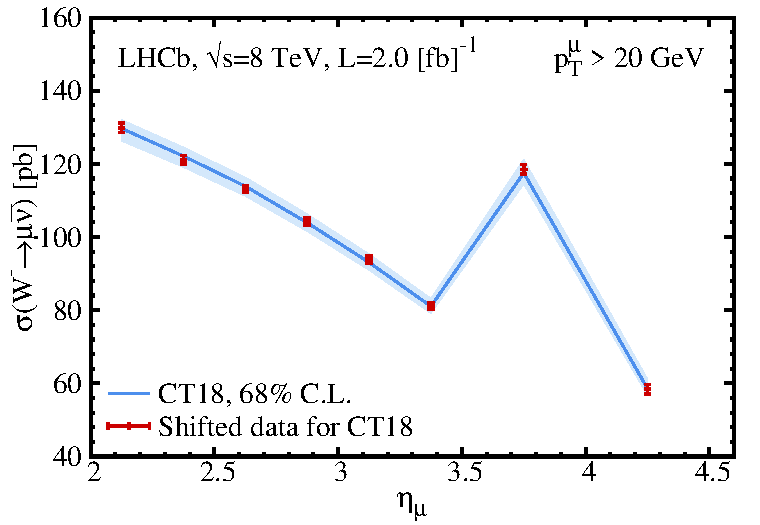
\includegraphics[width=0.49\textwidth]{./fig/data_250_CT18__2_abs_ect.pdf}
	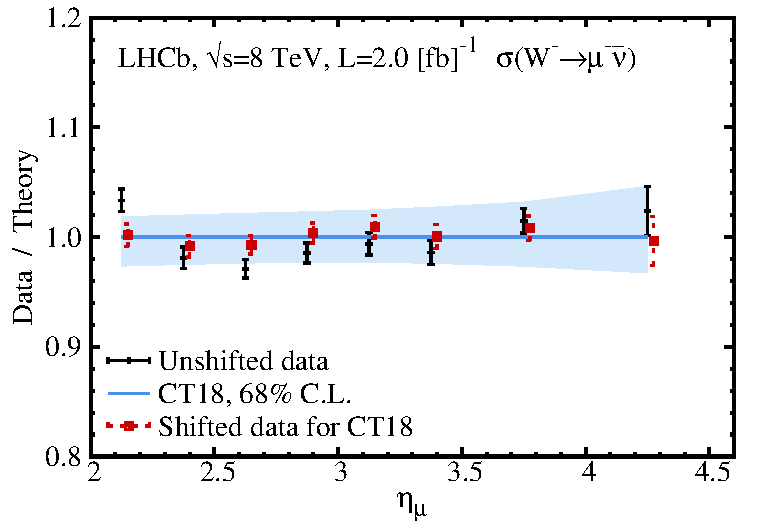
\includegraphics[width=0.49\textwidth]{./fig/data_250_CT18__2_DoT_ect.pdf}
	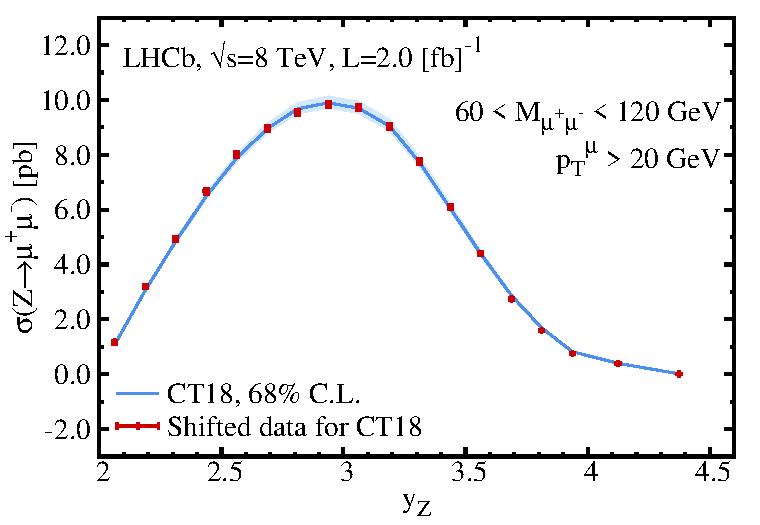
\includegraphics[width=0.49\textwidth]{./fig/data_250_CT18__3_abs_ect.pdf}
	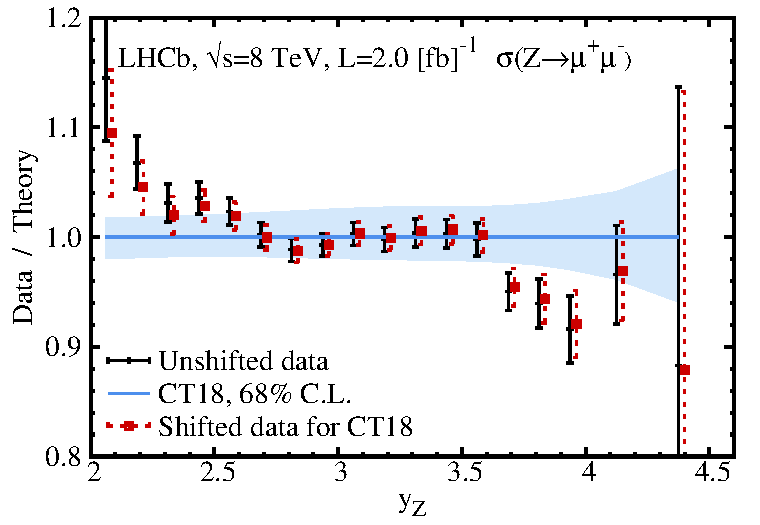
\includegraphics[width=0.49\textwidth]{./fig/data_250_CT18__3_DoT_ect.pdf}
	\caption{A comparison of the CT18 theoretical predictions to the $W^+$ (top), $W^-$ (middle), and $Z^0$ (bottom) cross section measurements by LHCb at 8 TeV in the muon decay channel (Exp.~ID=250). The data are presented as cross sections for each bin, $\sigma=\frac{d\sigma}{d\eta_\mu}\Delta\eta_\mu,\frac{d\sigma}{dy_Z}\Delta y_Z$, rather than as differential cross sections.
	The bump in the histogram bin $3.5<\eta_\mu<4.0$ of $W^-$ plot thus results from its larger bin width. A similar bump occurs in the plots for the LHCb 7 TeV $W/Z$ data (Exp. ID=245).
			\label{fig:id250}
}
\end{figure}

\begin{figure}[tb]
	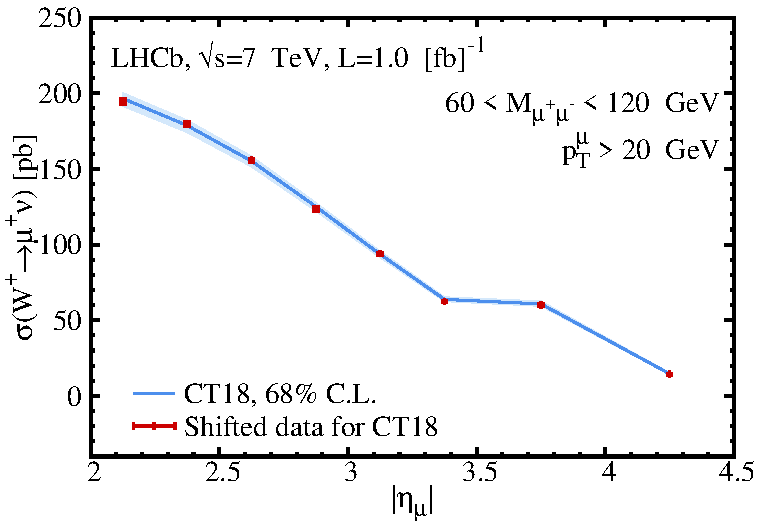
\includegraphics[width=0.49\textwidth]{./fig/data_245_CT18__2_abs_ect.pdf}
	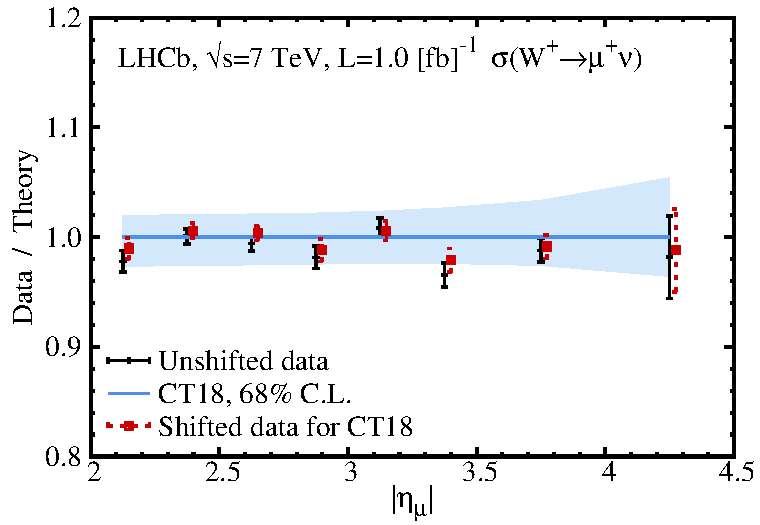
\includegraphics[width=0.49\textwidth]{./fig/data_245_CT18__2_DoT_ect.pdf}
	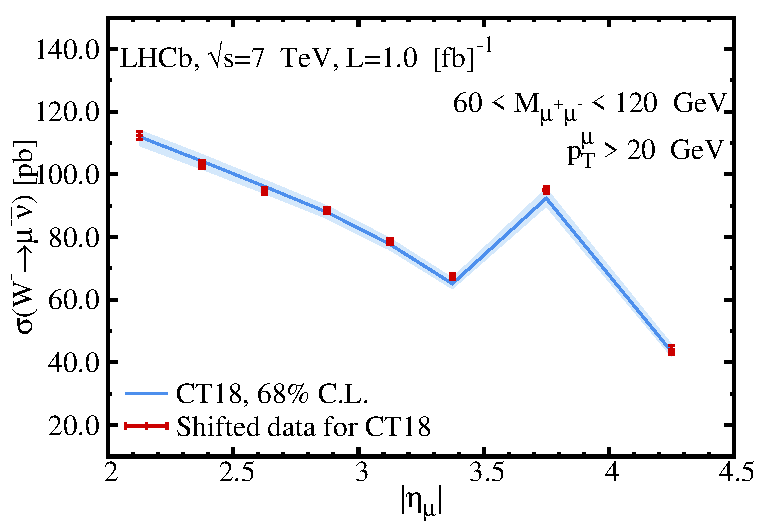
\includegraphics[width=0.49\textwidth]{./fig/data_245_CT18__3_abs_ect.pdf}
	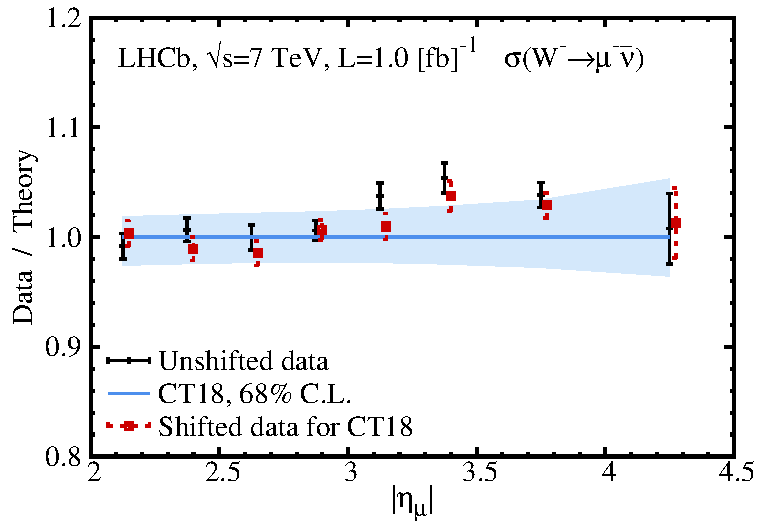
\includegraphics[width=0.49\textwidth]{./fig/data_245_CT18__3_DoT_ect.pdf}
	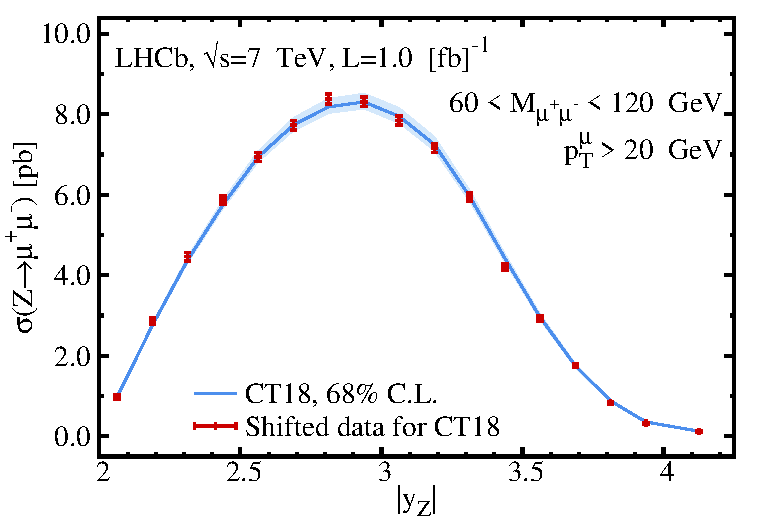
\includegraphics[width=0.49\textwidth]{./fig/data_245_CT18__1_abs_ect.pdf}
	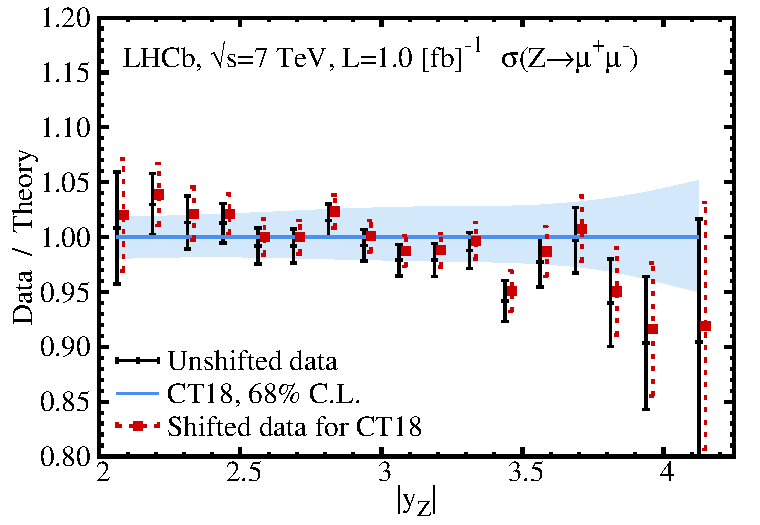
\includegraphics[width=0.49\textwidth]{./fig/data_245_CT18__1_DoT_ect.pdf}
	\caption{Same as Fig.~\ref{fig:id250}, for the LHCb 7 TeV (Exp.~ID=245).}
	\label{fig:id245}
\end{figure}


{\bf LHC data: LHCb.}
%
As discussed previously, Drell-Yan cross-section measurements from the LHCb collaboration (Exp.~IDs=250, 245 and 246, 
in that order of importance) produce the strongest impact on CT18 PDFs among the newly introduced LHC Drell-Yan data sets. Similarly to the D0 electron charge asymmetry, in Fig.~\ref{fig:id250}, 
the CT18 NNLO theory prediction is compared to both the shifted and the unshifted data of
$W/Z$ production  in the muon channel (Exp.~ID=250) at 8 TeV. 
The analogous comparisons to $W/Z$ production in the $\mu$ channel (Exp.~ID=245) at 7 TeV, and to $Z$ production in the $e$ channel (Exp.~ID=246) at 8 TeV are respectively shown in Fig.~\ref{fig:id245} and Fig.~\ref{fig:LHCb8Zee}.  
The NNLO theory is obtained using \texttt{APPLgrid} files generated with NLO \texttt{MCFM}, and multiplied by point-by-point $K$-factors computed 
with \texttt{FEWZ} and \texttt{MCFM-8.0}. 

In the case of $Z/W$ boson production at 8 TeV in Fig.~\ref{fig:id250}, 
theory and data agree well except for the data points near rapidity of 2. 
In $Z$ boson production in all three data sets (bottom rows), some disagreement between theory and data in shape at $y_Z <2.5$ and $y_Z=3-4$ remains in spite of systematic shifts. It leads to the  elevated $\chi^2_E$ for experiments 245 and 250 quoted in Table \ref{tab:EXP_2}, the discrepancy that is partially alleviated in the CT18Z fit after including the ATLAS 7 TeV $W/Z$ production data set (Expt.~ID=248).
At low rapidity in $Z$ production, there is a large modeling uncertainty for the kinematic acceptance of the observed leptons. 
On the other hand, the discrepancy at $y_Z\approx 4$ shows tension with pulls from other data sets included in the global fit, 
such as the CMS and D0 $W$ lepton-charge asymmetry data. This tension has been investigated using the \texttt{ePump} program. In particular, we compared updated fits in which we either had included, or had not included, the first (low rapidity) bin of the $Z$-boson distribution for Experiment 246. This choice had little impact on the resulting PDFs, though the $\chi^2_E/N_{pt,E}$ of the LHCb data had noticeably improved after dropping the first rapidity bin. 

The quality of the CT18 fit to the individual data points can be quantified by the histograms of the shifted residuals
shown in Fig.~\ref{fig:res_rk_1}. When the fit to experiment $E$ is good, the histograms of its shifted residuals $r_i\! =\! (D^\mathit{sh}_{i}-T_{i})/s_{i}$  and optimized nuisance parameters $\bar\lambda_\alpha$ are consistent with the standard normal distribution. For example, the third panel  illustrates the distribution of $r_i$ for
the LHCb 8 TeV $W^\pm$ and $Z$ data (Exp.~ID=250). It indicates that there are 
a few data points with large values in the Exp.~ID=250 data set. As expected, the large residuals result from the first 
few rapidity bins near $y=2$ in the $W^\pm$ and $Z$ data, and from $3.5\lesssim y_Z\lesssim 4$ between 3.5 and 4 in the $Z$ data.
%
%\textcolor{red}{Can we explain the discrepancy for $y$ between 3.5 and 4 nin $Z$ data?}
%
Another useful criterion is the examination of the distribution of nuisance parameters needed 
to fit the Exp.~ID=250 data, which is shown in the left Fig.~\ref{fig:res_rk_3}. The distribution of nuisance parameters deviates from the normal distribution, with two nuisance parameters having particularly large values ($-3$ and $+3.7$).
The right panel of Fig.~\ref{fig:res_rk_3} represents 
the $L_2$ sensitivity of these data to various PDF flavors at $Q=100$ GeV. We see that the LHCb data prefers lower $u$, $\bar u$ PDFs at $x<10^{-2}$, as compared to the full global data, somewhat higher $s$ at $x < 10^{-2}$, and a higher $\bar d$ at $x\approx 0.2$. The plots of $L_2$ sensitivities for the other experiments and PDF combinations can be viewed at Ref.~\cite{CT18L2Sensitivity}.

\begin{figure}[p]
\includegraphics[width=0.49\textwidth]{./fig/fig2/data_246_CT18_abs_ect.pdf}
\includegraphics[width=0.49\textwidth]{./fig/fig2/data_246_CT18_DoT_ect.pdf}
\caption{A comparison of the CT18 theoretical predictions to the $Z$ rapidity distribution in $Z\to e^+e^-$ production by LHCb at 8 TeV (Exp.~ID=246) .
}
\label{fig:LHCb8Zee}
 \end{figure}

\begin{figure}[t]
	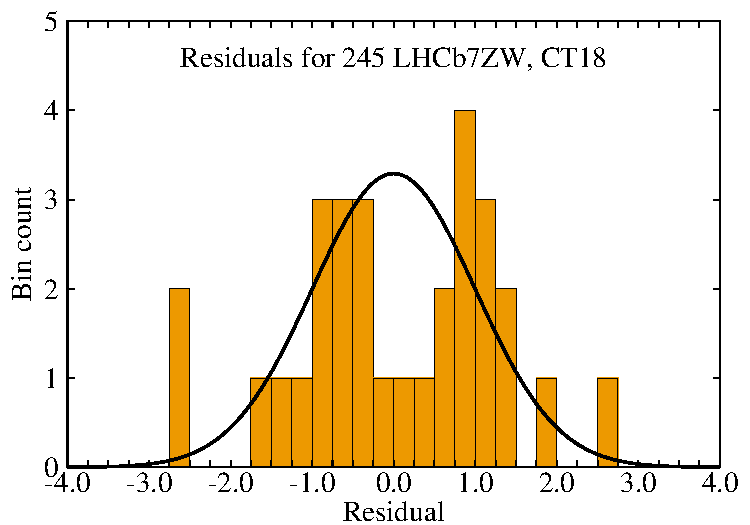
\includegraphics[width=0.32\textwidth]{./fig/res_his_CT18-245_4_ect.pdf}
	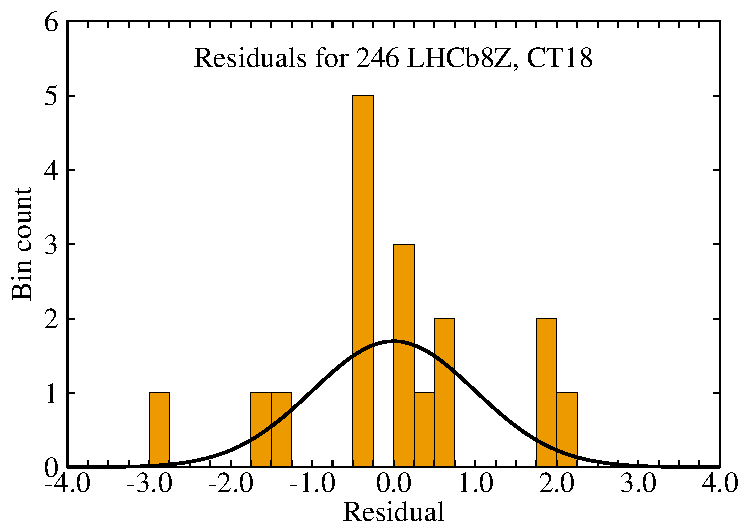
\includegraphics[width=0.32\textwidth]{./fig/res_his_CT18-246_4_ect.pdf}
	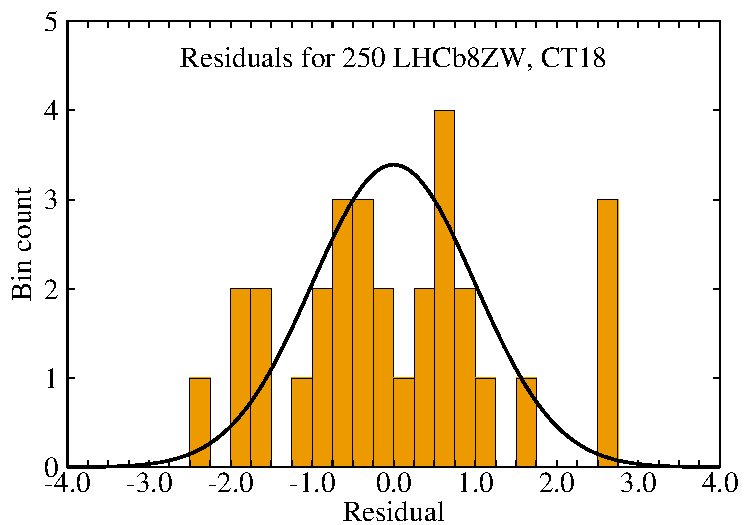
\includegraphics[width=0.32\textwidth]{./fig/res_his_CT18-250_4_ect.pdf}
	\caption{Distributions of the residuals for the LHCb $W/Z$ production cross sections at 7 and 8 TeV: Exp.~ID=245 (left), 246 (center), and 250 (right).
		\label{fig:res_rk_1}}
\end{figure}



\begin{figure}[t]
	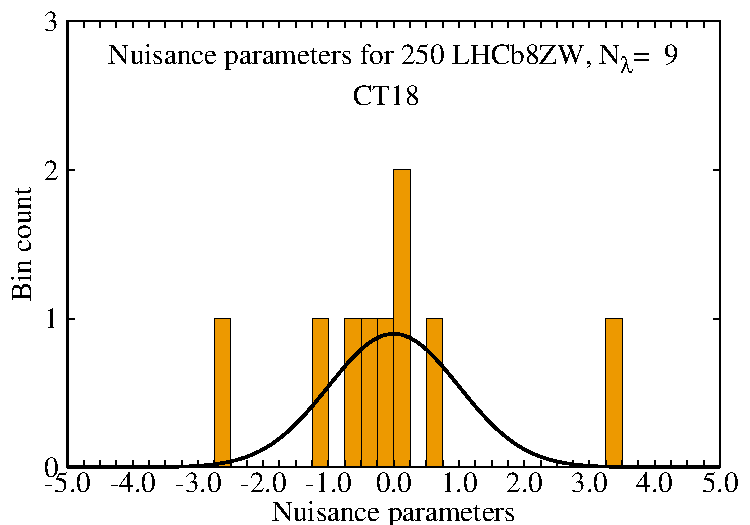
\includegraphics[width=0.45\textwidth]{./fig/rk_his_CT18-250__4_ect.pdf}\quad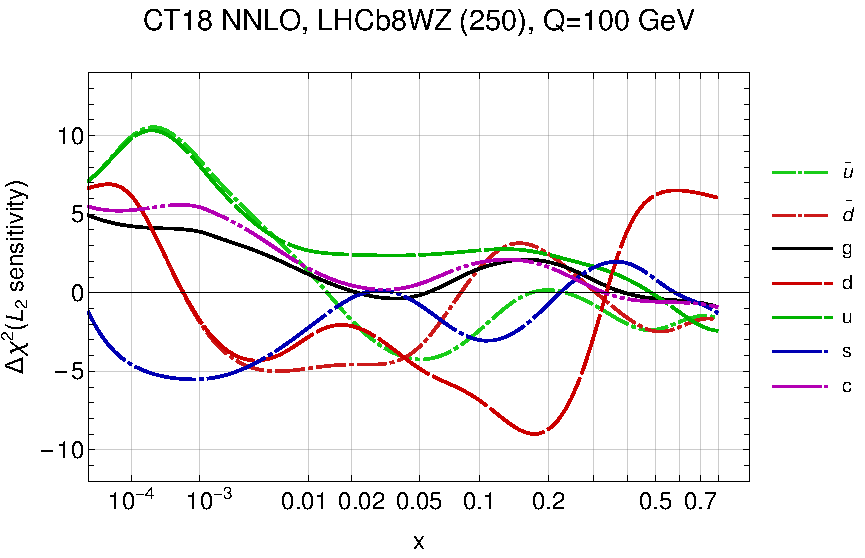
\includegraphics[width=0.53\textwidth]{./fig/250_CT18_L2_Q100.pdf}
	\caption{Left: distribution of nuisance parameters for the LHCb 8 TeV $W/Z$ cross sections (Exp.~ID=250).\\ Right: the pulls of these data on the CT18 NNLO PDFs at $Q=100$ GeV, computed in terms
of the $L_2$ sensitivity of Eq.~(\ref{eq:L2}) \cite{CT18L2Sensitivity}.
		\label{fig:res_rk_3}}
\end{figure}


%\begin{figure}[t]
%\caption{
%}
%\label{fig:corr_250}
%\end{figure}



%\begin{figure}[htbp]
%	\includegraphics[width=0.49\textwidth]{./fig/data_246_CT18_abs_ect.pdf}
%	\includegraphics[width=0.49\textwidth]{./fig/data_246_CT18_DoT_ect.pdf}
%	\caption{A comparison of the CT18 theoretical predictions to the LHCb 8 TeV $Z$ rapidity data (Expt. ID 246)
%	{\bf Tim: the theory calculation did not include
%	K-factors; fix and update plots}. \textcolor{red}{KP: attention, this data is differential cross section, different from 245 and 250.}
%		 }
%\end{figure}



%
% - - - - - - - - - - - - - - - - - - - - - - - - - - - - - - - - - - - - - - - - - - - - - - - - - - - - - - - - - - - - - - - - - - - - - - - - -
%
{\bf LHC data: CMS and ATLAS.}
Measurements of lepton charge asymmetry at 8 TeV (Exp.~ID=249) from the CMS collaboration are included  
in all the CT18 global fits. The theoretical predictions, compared with the shifted 
and unshifted data, are shown in Fig.~\ref{fig:id249}. We see that all the 
experimental data are fitted well within the 68\% C.L. PDF uncertainty.  


%For the ATLAS 8 TeV $Z$-$p_T$, We have dropped the low-$p_T$ data due to the missing resummation effect in our fixed-order calculation. The ATLAS 8 TeV $Z$-$p_T$ data (Expt. ID 253) will receive contributions EW corrections. We have conducted a detailed investigation, which shows that the negative EW corrections cancel the photon-induced (PI) contribution to a large extent. It validates the NNLO QCD calculation used in our PDF fitting. We will come back to the details in the next subsection.

%%%%%%%%%%%
%\textcolor{red}{Only show the shifted data in the left-panel plots. The errors bars of un-shifted and shifted data need to be checked. }

% CMS
\begin{figure}[t]
	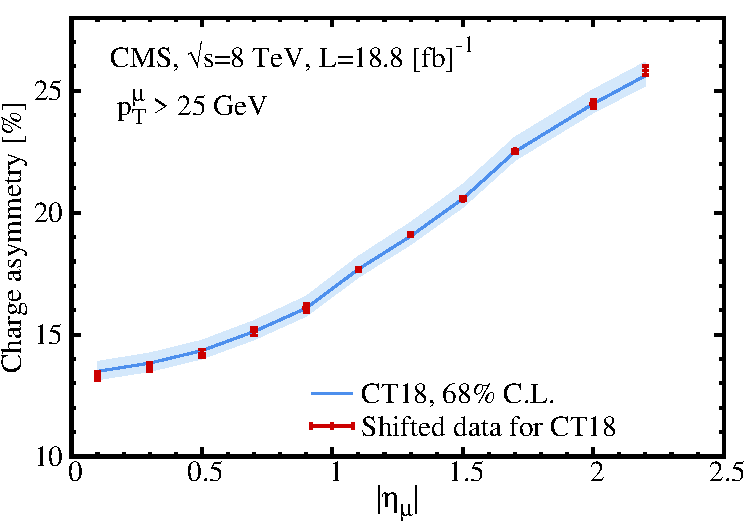
\includegraphics[width=0.49\textwidth]{./fig/data_249_CT18_abs_ect.pdf}
	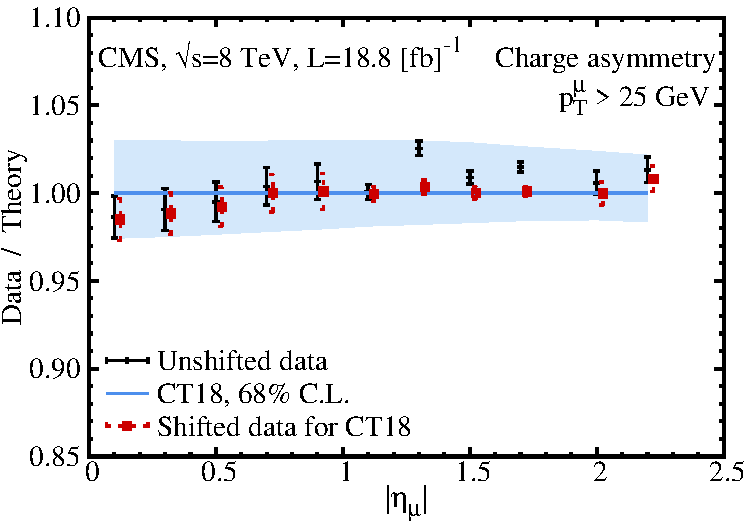
\includegraphics[width=0.49\textwidth]{./fig/data_249_CT18_DoT_ect.pdf}
	\caption{A comparison of the CT18 theoretical predictions to the CMS 8 TeV charge asymmetry data (Exp.~ID=249).}
\label{fig:id249}
\end{figure}


%ATLAS
%\begin{figure}[htbp]
%	\includegraphics[width=0.49\textwidth]{./fig/data_251_CT18_abs_ect.pdf}
%	\includegraphics[width=0.49\textwidth]{./fig/data_251_CT18_DoT_ect.pdf}
%	\caption{A comparison of the CT18 theoretical predictions to the ATLAS 8 TeV high mass Drell-Yan data (Expt. ID 251).}
%\label{fig:id251}
%\end{figure}


% ATLAS 8TeV ZpT data
\begin{figure}[t]
	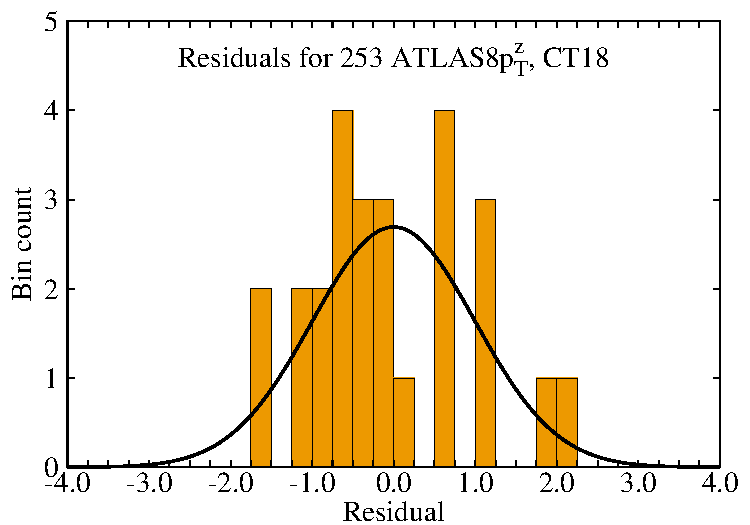
\includegraphics[width=0.49\textwidth]{./fig/res_his_CT18-253_4_ect.pdf}
	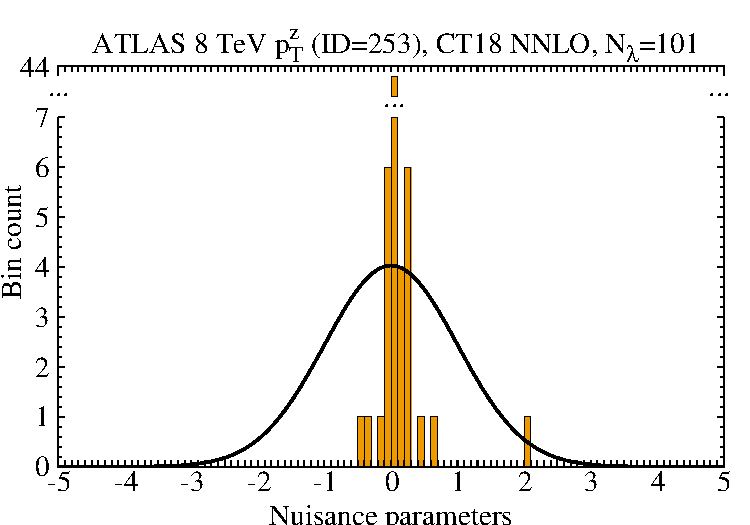
\includegraphics[width=0.49\textwidth]{./fig/rk_his_CT18-253_10_v3_ect.pdf}	
	\caption{Distribution of residuals (left) and nuisance parameters (right) for the ATLAS 8 TeV $Z$ $p_T$ data in their mass bins, with Exp.~ID=253. A large number of the $N_\lambda\! =\! 101$ nuisance parameters are $\sim\! 0$, and we abbreviate the
	vertical scale in the right panel to highlight the large $\lambda_\mathrm{lumi}\! =\! 2.02$ nuisance parameter associated with the luminosity uncertainty.
		\label{fig:res_rk_6}}
\end{figure}

\begin{figure}[t]
\includegraphics[width=0.49\textwidth]{./fig/data_253_CT18__1_abs_ect.pdf}
\includegraphics[width=0.49\textwidth]{./fig/data_253_CT18__1_DoT_ect.pdf}
\includegraphics[width=0.49\textwidth]{./fig/data_253_CT18__2_abs_ect.pdf}
\includegraphics[width=0.49\textwidth]{./fig/data_253_CT18__2_DoT_ect.pdf}
\includegraphics[width=0.49\textwidth]{./fig/data_253_CT18__3_abs_ect.pdf}
\includegraphics[width=0.49\textwidth]{./fig/data_253_CT18__3_DoT_ect.pdf}
\caption{A comparison of the CT18 theoretical predictions to the ATLAS 8 TeV $Z\, p_{T}$ data (Exp.~ID=253). Predictions for the $p_T$ spectra measured by the ATLAS in
3 bins of the dilepton invariant mass,
$46\! <\! M_{ll}\! <\! 66$ GeV,
$66\! <\! M_{ll}\! <\! 116$ GeV, and
$116\! <\! M_{ll}\! <\! 150$ GeV, are shown in the upper, center, and lower rows, respectively.
The right panels give the corresponding $\mathrm{Data}/\mathrm{Theory}$ profiles
for these data.
\label{fig:id253}}
\end{figure}
%


In the CT18(Z) analysis, we have also included the transverse momentum ($p_{T}$) 
distributions of lepton pairs produced in $Z$ decays at ATLAS at 
$\sqrt{s}=8$ TeV (Exp.~ID=253).
The theoretical predictions for these data are obtained based on the NNLO fixed-order 
calculations for $Z+$jet production. 
We stress that we have imposed a kinematic cut $45<p_T^Z<150$ 
GeV to remove the low- and high-$p_T$ regions where this fixed-order calculation lacks the necessary accuracy.  The low-$p_T$ data are dropped 
because of the missing resummation effects in our fixed-order calculation. 
The high-$p_T$ data are dropped because (1) the constraining power of the data is small given the relatively large statistical errors, and (2) the EW corrections are non-negligible, 
as will be discussed in Sec.~\ref{sec:EW}.

As a practical implementation, we generated in-house NLO \texttt{APPLgrid} files with \texttt{MCFM} and multiplied them by the NNLO/NLO $K$-factors computed as the ratios of the NNLO and NLO cross sections published in
Refs.~\cite{Ridder:2015dxa,Gehrmann-DeRidder:2017mvr,Gehrmann-DeRidder:2016jns,Gehrmann-DeRidder:2016zml,Ridder:2016rzm,Ridder:2016nkl}.
To account for non-negligible fluctuations in the NNLO theoretical prediction, we have included an additional 0.5\% theoretical Monte-Carlo uncertainty, estimated by the standard deviation for a smooth-curve fitted to discrete $K$-factors.
The renormalization and factorization scales are chosen as
%
\begin{equation}
\mu_{R}=\mu_{F}=M_{T}^{ll}=\sqrt{(p_{T}^{ll})^{2}+M_{ll}^{2}}\; .
\end{equation}
The CT18 NNLO theoretical predictions are compared to the ATLAS 8 TeV data in Fig.~\ref{fig:id253}. 
We see that, for CT18 NNLO to describe the data in all 3 invariant-mass bins, substantial systematic shifts are required.
The distributions of the residuals and nuisance parameters of these data are shown in Fig.~\ref{fig:res_rk_6}.
There is an overall systematic shift when comparing the unshifted data to the 
theoretical predictions in Fig.~\ref{fig:id253}. The corresponding nuisance parameter 
associated with this shift, due to the luminosity error, is $\lambda_\mathrm{lumi}\! =\!2.02$, as can be seen in the upper tail of the distribution plotted
in the right panel of Fig.~\ref{fig:res_rk_6}.
We have investigated the scale dependence by varying the renormalization and 
factorization scales independently by a factor of 2, while restricting their ratio to be
\begin{equation}
\frac{1}{2}\leq\frac{\mu_{R}}{\mu_{F}}\leq 2\;.
\end{equation}
%
We find that the optimal scale choice to describe the unshifted data is given by
%
\begin{equation}
\mu_{R}=M_{T}^{ll}/2, ~\mu_{F}=M_{T}^{ll}\;.
\end{equation}
With this scale choice, the unshifted data for the $Z$ mass range are 
located around the margin of 1$\sigma$ theoretical uncertainties, as shown in Fig. \ref{fig:ATL8ZpT}. 
%

\begin{figure}[p]
\begin{center}
\includegraphics[width=0.42\textwidth]{./fig/fig2/CT18-7_CT18Z-7_CT14H-7_1_mll1.pdf}
\includegraphics[width=0.42\textwidth]{./fig/fig2/CT18-7_CT18Z-7_CT14H-7_2_mll2.pdf}
\includegraphics[width=0.42\textwidth]{./fig/fig2/CT18-7_CT18Z-7_CT14H-7_3_mll3.pdf}
\caption{Theoretical predictions based on the CT14$_\mathrm{HERAII}$, CT18, and CT18Z NNLO PDFs for lepton pair transverse momentum distribution, $p^{ll}_T$, compared with the ATLAS 8 TeV measurements. The yellow band represents the PDF uncertainties calculated with the symmetric Hessian method at the 68\% C.L. The dashed band represents the scale uncertainty. }
\label{fig:ATL8ZpT}
\end{center}
\end{figure}

The remaining difference cannot be explained by the %missing we don't use them for W/Z data??
EW corrections, 
since the EW corrections are small and negative (see Sec.~\ref{sec:EW}), 
pulling the theory further away from the data. Instead, the systematic shift in the normalization can possibly be ascribed to the missing higher-order (N$^{3}$LO) corrections, implied by two observations. First, the NNLO corrections to the $Z$ $p_{T}$ are generally as large as 10\%, which indicates 
slow convergence of the perturbative expansion. Second, the large 
scale uncertainty (about 3-4\%) is also an indication that the missing 
higher-order effects may be significant.


\subsubsection{Jet data}
\label{sec:Jet_fit}
%
%
Historically, inclusive jet production has played an important role in constraining the gluon density, $g(x,\Q)$, as evidenced by the impact that the older jet data from the Tevatron Run-II had on the CT10 and CT14 global analyses.  CT18 now also implements inclusive jet production data at even higher collider energies and  luminosities, measured by the ATLAS and CMS collaborations at the LHC, as described in Sec.~\ref{sec:DataJets}.

{\bf Tevatron Run-II data.}
%
%
First, we examine the fits to the Tevatron Run-II jet data. 
The CDF Run-II 
data shown in Fig.~\ref{fig:id504} is not perfectly described by NNLO theory (has an elevated $\chi^2_E/N_{pt,E}\approx 1.7$ according to Table~\ref{tab:EXP_1}) and prefers a somewhat different shape of the gluon PDF $g(x,Q)$, compared to the average of all experiments, according to the $L_2$ sensitivity plot for $g(x,Q)$ in Fig.~\ref{fig:L2glu}. The D0 Run-II jet data, depicted in Fig.~\ref{fig:id514}, show better agreement with the rest of the data sets.

% Tevatron Jets
\begin{figure}[b]
	\includegraphics[width=1.0\textwidth]{./fig/data_504_CT18__com_DoT_hori_ect.pdf}
	%\includegraphics[width=0.8\textwidth]{./fig/data_504_CT18__com_DoT_vert_ect.pdf}
	\caption{$\mathrm{Data}/\mathrm{Theory}$ values for CT18 NNLO and CDF Run 2 jet data (Exp.~ID=504).
		 \label{fig:id504}}
\end{figure}

\begin{figure}[p]
	\includegraphics[width=1.0\textwidth]{./fig/data_514_CT18__com_DoT_hori_ect.pdf}
	%\includegraphics[width=0.8\textwidth]{./fig/data_514_CT18__com_DoT_veri_ect.pdf}
	\caption{$\mathrm{Data}/\mathrm{Theory}$ values for CT18 NNLO and D0 Run-2 inclusive jet production (Exp.~ID=514).
	     \label{fig:id514}}
	
\end{figure}


%
{\bf Run-1 LHC data.}
%
%
The CT18 fit can describe the LHC CMS and ATLAS jet data, depicted in Figs.~\ref{fig:DoT542}-\ref{fig:DoT545},
after the decorrelation of some correlated systematic errors, as 
laid out in Sec.~\ref{sec:DataJets} and App.~\ref{sec:ATLASjetdecorrel}, 
as well as the inclusion of a $0.5\%$ overall uncorrelated 
systematic error for all the LHC jet data,
as discussed in Sec.~\ref{sec:DataJets}.

%
Although the agreement with theory in the CT18 analysis is reasonable, 
we note some tensions among the LHC inclusive jet data sets themselves, especially the CMS 
results at 7 (Exp.~ID=542) and 8 TeV (Exp.~ID=545).
%
These tensions are particularly pronounced for some parton flavors in the specific kinematic regions --- most evidently, for the gluon PDF, as
quantified by the LM scans and $L_2$ sensitivity profiles plotted 
in Figs.~\ref{fig:LMg18} and~\ref{fig:L2glu}, respectively.
For the ATLAS inclusive jet data at 7 TeV, the best fit requires
the correlated errors to shift the raw data downward
in the smaller rapidity regions, but to shift the raw data upward at high rapidities. The majority of optimal nuisance 
parameters $\lambda_{\alpha}$ for the CT18 NNLO PDF set, shown in the histograms included in the supplementary material, are distributed 
narrowly about $|\lambda_{\alpha}|\! \sim\! 0$. For the CMS 8 TeV data set, four nuisance parameters out of 28 require absolute correlated shifts larger than two -- a larger count than is expected based on the assumed normal statistics. 


%
\begin{figure}[p]
\includegraphics[width=1.0\textwidth]{./fig/data_542_CT18__com_DoT_hori_ect.pdf}
\caption{$\mathrm{Data}/\mathrm{Theory}$ values for CT18 NNLO and  CMS 7 TeV inclusive jet production (Exp.~ID=542).
\label{fig:DoT542}
}
\end{figure}
%
\begin{figure}[p]
\includegraphics[width=1.0\textwidth]{./fig/data_544_CT18__com_DoT_hori_ect.pdf}
\caption{$\mathrm{Data}/\mathrm{Theory}$ values for CT18 NNLO and ATLAS 7 TeV inclusive jet production (Exp.~ID=544).
\label{fig:DoT544}
}
\end{figure}
%
\begin{figure}[p]
\includegraphics[width=1.0\textwidth]{./fig/data_545_CT18__com_DoT_hori_ect.pdf}
\caption{$\mathrm{Data}/\mathrm{Theory}$ values for CT18 NNLO and CMS 8 TeV inclusive jet production (Exp.~ID=545).
\label{fig:DoT545}
}
\end{figure}


\subsubsection{Top-quark pair production data
\label{sec:QualityTopData}
}


The two $t\bar{t}$ data sets included in the CT18 global analysis are well-described, as shown by the values of $\chi^2$ and effective Gaussian variable $S_E$ 
given in the latter two rows of Table~\ref{tab:EXP_2}. 
In particular, for the CMS (Exp.~ID=573) and ATLAS (Exp.~ID=580) data sets included in the fit,
we obtain $S_E\! =\! 0.6$ and $S_E\! =\! -1.1$, respectively.
For a detailed point-by-point description of the $t\bar{t}$ agreement with the theory,
in Figs.~\ref{fig:573} and~\ref{fig:580} we show plots of 
the $(\mathrm{Data})/(\mathrm{Theory})$ ratio
for both data sets.
%
Error bars were calculated by including both statistical and 
correlated systematic errors listed in Tables 5 and 7 of Ref.~\cite{Sirunyan:2017azo}. 
We have checked that including the covariance matrix of statistical 
correlated uncertainties (listed in Table 6 of Ref.~\cite{Sirunyan:2017azo}), via \texttt{ePump} updating, does not further modify the resulting PDFs. (See Ref.~\cite{Czakon:2019yrx} for detailed discussion.)
%

%t-tbar
\begin{figure}[h]
	\includegraphics[width=0.7\textwidth]{./fig/data_573_CT18__com_DoT_ect.pdf}
	\caption{$(\mathrm{Data})/(\mathrm{Theory})$ comparison for the
	CMS 8 TeV $t\bar{t}$ production data (Exp.~ID=573) as a function of the transverse momentum of the top (anti-)quark.}
\label{fig:573}
\end{figure}

\begin{figure}[h]
	\includegraphics[width=0.49\textwidth]{./fig/data_580_CT18__1_DoT_ect.pdf}
	\includegraphics[width=0.49\textwidth]{./fig/data_580_CT18__2_DoT_ect.pdf}
	\caption{$(\mathrm{Data})/(\mathrm{Theory})$ comparison for the
	ATLAS 8 TeV $t\bar{t}$ production data (Exp.~ID=580) as a function of the $t\bar t$ invariant mass.}
\label{fig:580}
\end{figure}


In Fig.~\ref{fig:573}, the top-quark $p_T$ distribution at CMS  
is fitted reasonably well across the four rapidity bins examined here. We find
modest deviations between theoretical predictions and the (un)shifted data
for some points in the intermediate rapidity bins, $0.75\! <\! |y_t| \! <\! 0.85$
and $0.85\! <\! |y_t| \! <\! 1.45$, contributing to the somewhat broader
distribution of residuals. Notably, the effect of correlated errors
in fitting the CMS data is relatively minimal, given the fact that the shifted (red) and unshifted (black) data are very similar, as observed in  Fig.~\ref{fig:573}. 
Correlated systematics are nonetheless important for some cross section values, allowing the data values to shift enough to be within 
$1\sigma$ distance from the CT18 prediction.

In contrast, achieving a very good description of the analogous ATLAS 
$p_{T,t}$ and $m_{t\bar{t}}$ distributions shown in Fig.~\ref{fig:580}
critically depends on the use of nuisance parameters to compensate for
correlated systematics, as seen in Fig.~\ref{fig:580}. 
%pn 2020-02-17
The uncorrelated errors are small (less than 1-2 percent) in most bins of this data set. In contrast, the systematic errors are sizable, the systematic shifts lead to a very good agreement between theory and data, with $\chi^2_E/N_{pt,E}=9.4/15$ for CT18 NNLO.


%
% ~ ~ ~ ~ ~ ~ ~ ~ ~ ~ ~ ~ ~ ~ ~ ~ ~ ~ ~ ~ ~ ~ ~ ~
%

\subsubsection{Dimuon production
\label{sec:Qualitydimuon}}

\NOTEPN{200430 Merged in Marco's changes. Need to read the subsection
  carefully.}
\NOTE{JG: I've rearranged sentences a little bit and clean out all comments.}

Charm-quark production cross sections in neutrino deep-inelastic scattering provide key low-$Q$ constraints on the strangeness PDF at $x > 10^{-2}$.
In the CT14 NNLO analyses, the charm-quark production cross section were calculated at NLO in
QCD~\cite{Gottschalk:1980rv,Gluck:1997sj,Blumlein:2011zu} in the S-ACOT-$\chi$ variable-flavor-number (VFN)scheme ~\cite{Aivazis:1993kh,Collins:1998rz,Kramer:2000hn,Tung:2001mv}.
Recently, charged-current coefficient functions in DIS have been calculated
to NNLO in QCD, including quark mass dependence ~\cite{Berger:2016inr,Gao:2017kkx}.
This calculation, in a fixed-flavor-number (FFN) scheme with 3 light-quark flavors,  is published in the form of fast interpolation tables for the kinematics of the CCFR and NuTeV dimuon experiments~\cite{Goncharov:2001qe,Mason:2006qa}.


The CT18 analysis still uses a NLO theory prediction in the S-ACOT-$\chi$ VFN scheme because
a consistent treatment of charm-quark mass effects at NNLO
in the CT framework requires matching of the theory prediction for the charged-current cross section in the FFN scheme to an ACOT-like VFN scheme, which is not yet available.
However, the NLO calculation for charged currents in the S-ACOT-$\chi$ VFN adopted in the CT18/18Z global analyis
can still be trusted within the current accuracy of the measurements.\footnote{We note the CCFR and NuTeV collaborations computed a significant acceptance correction to extract the charm-quark production cross sections from dimuon cross sections using a Monte Carlo generator with NLO precision only.}
%
Besides, the discussion in Ref.~\cite{Gao:2017kkx} indicates that, for the kinematics of CCFR and NuTeV, the differences between the NNLO results from the FFN scheme and any VFN scheme are expected to be significantly smaller than the precision of experimental data.

	\begin{figure}[b]
		\begin{center}
			\includegraphics[width=0.47\textwidth]{fig/CT18dimuonalts1_KP.pdf}\hspace{0.1in}
			\includegraphics[width=0.47\textwidth]{fig/CT18Zdimuonalts1_KP.pdf}
			\includegraphics[width=0.47\textwidth]{fig/CT18dimuonalts2_KP.pdf}\hspace{0.1in}
			\includegraphics[width=0.47\textwidth]{fig/CT18Zdimuonalts2_KP.pdf}
		\end{center}
		\vspace{-2ex}
		\caption{\label{fig:dimuonalt}
			%
			Strange-quark distribution $s(x,Q)$  and ratio $R_s(x,Q)$ in CT18 (left) and
			CT18Z (right) NNLO fits, compared with alternative fits using QCD NNLO cross sections for CCFR and NuTeV measurements.
		}
	\end{figure}
	

As a cross check, we have carried out alternative fits, labeled CT18(Z)-charmDIS NNLO, using the NNLO FFN calculations for dimuon production cross sections. 
In the case of CT18-charmDIS NNLO, the global $\chi^2$ is reduced by 6 units (compared to CT18), with the reduction in the $\chi^2_E$ for the dimuon data of the order of 1-2 units.
%
For CT18Z-charmDIS NNLO, the global $\chi^2$ and the $\chi^2_E$ for the dimuon data  are reduced by 11 and 8 units, respectively, compared to CT18Z.
In both cases the NNLO predictions  provide a marginally better agreement with the data. 

The impact of these choices  on the strange-quark PDF has also been cross checked. The strange-quark PDF $s(x,Q)$ and the ratio $R_s(x,Q)$ defined in Eq.~(\ref{eq:Rs}) are compared in
Fig.~\ref{fig:dimuonalt} for the nominal CT18(Z) fits and their ``charmDIS NNLO'' alternatives. 
%
In the
CT18-charmDIS fit, we observe a slight increase of the strange-quark PDF at $x\! \approx\! 0.1$. This outcome is consistent with the PDF profiling results in Ref.~\cite{Gao:2017kkx} and reflects negative NNLO QCD corrections in the same $x$ region. In the CT18Z-charmDIS fit, with the ATLAS 7 TeV
$W/Z$ data included, the PDFs change less as compared to the CT18-charmDIS fit.
%
Furthermore, the changes due to the NNLO contribution to dimuon production are small compared to the size of the PDF uncertainties, as one
can also infer from the relative stability of the $\chi^2$ values for the nominal and alternate fits.
%


\begin{figure}[htbp]
	\includegraphics[width=0.8\textwidth]{./fig/pdfs_CT14HERA2dimuons.pdf}
	\caption{\label{fig:epump-dimuon}
		Comparison of $s$ PDF at $Q=100$ GeV for various fits. See the main text for its detail. }
\end{figure}

The tendency of the NNLO corrections to the dimuon cross sections to slightly increase the strangeness to higher values at $x\! \approx\! 0.1$ has  independently been confirmed by using the fast Hessian updating technique with \texttt{ePump}~\cite{Hou:2019gfw}, as well as by the MMHT group~\cite{Thorne:2019mpt}, cf.~Appendix~\ref{sec:AppendixCT18Z}.

Finally, to estimate the impact of the NNLO corrections to the charm-quark production cross section on the simultanous inclusion of the ATL7ZW and dimuon data sets,
we performed a series of NNLO fits illustrated in Fig.~\ref{fig:epump-dimuon}. There, we compare the strange-quark PDF obtained 
from four different fits that have been updated with \texttt{ePump}. PDF set (1)
is the base fit obtained from the \CTHERAII~data set by removing
the NuTeV and CCFR dimuon data. 
Adding back those four dimuon data sets, with NLO and NNLO predictions, yields the sets (2) and (3), respectively. PDF set (4) is obtained 
by adding the ATL7ZW data set, without the dimuon data sets. 
While PDF set (3) [found using the NNLO dimuon cross sections] yields an $s$ PDF that is marginally closer to
that constrained by the  ATL7ZW data for $10^{-3}\! \lesssim\! x\! \lesssim\! 10^{-1}$,  the improvement is still too weak to resolve the tension between the 
ATL7ZW and dimuon data sets.

%\NOTE{MG, PN -- optional} Concluding, we have performed a series of
%extensive cross checks on the current NLO theory calculation for DIS
%charged currents in CT18 and we have shown that this calculation is
%still trustworthy within the current accuracy of the measurements
%included in the fit. 

\subsection{Electroweak corrections}
\label{sec:EW}
%
%

\begin{table}
\caption{A summary of electroweak corrections to the LHC precision data considered for CT18(Z).  For each process, we indicate the primary observable, an approximate upper bound
for the EW correction, references for computing the EW corrections, and whether the data were adopted in CT18(Z) with or without EW corrections.}
\label{tab:EWcorrections}
\hspace*{-0.75cm}\begin{tabular}{c|c|c|c|c|c}
\hline
\multirow{2}{*}{Data} & \multirow{2}{*}{Observables}  & Size of EW (and PI)  & Ref. & Data included & EW corrections  \\
 &    & corrections & & in the CT18(Z)? & included in the fits\\
\hline
	Inclusive jet & $p_{T}\sim1.4$ TeV, central  & 8\%  & \cite{Dittmaier:2012kx} & Yes & Yes \\
\hline
	$t\bar{t}$ &$p_{T}^{t}\sim500$ GeV   &  -5\% & \cite{Czakon:2017wor} & Yes & No \\
\hline
$W^{+}(W^{-})$ &     & -0.4(0.3)\%  & \multirow{4}{*}{\cite{Aaboud:2016btc}} & \multirow{4}{*}{CT18Z} & \multirow{4}{*}{Yes}  \\
DY low-mass & $46<M_{ll}<66$ GeV central  & +1.5\%(PI) +6\%(EW) &  &     \\
DY $Z$-peak  & $66<M_{ll}<116$ GeV central (forward) & $<$0.1\%(PI)-0.3(-0.4)\%(EW)  & & \\
DY high-mass &$116<M_{ll}<150$ GeV central (forward) & +1.5\%(PI)-0.5(-1.2)\% (EW) & & \\
\hline
high-mass Drell-Yan & $M_{ll}\sim1$ TeV  & +5\%(PI)-3\%(EW)  & \texttt{FEWZ} & No  & -- \\
\hline
\multirow{2}{*}{$Z$ $p_{T}$} & $p_{T}\sim m_Z$ & about -5\%   & \cite{Kallweit:2015fta} & Yes & No \\
 & $p_{T}\sim1$ TeV & about -30\%   & \cite{Kallweit:2015fta} & No & --  \\
\hline
\end{tabular}
\end{table}

In this subsection, we present a  summary of the electroweak (EW) corrections for the LHC data which were considered, and,
in some cases, applied, to the CT18(Z) fits. In general, we have not used data for which EW corrections are large, especially
if the data do not provide significant constraints to the PDFs. EW corrections tend to be larger in those kinematical regions
for which the statistical errors of the data are also sizable, such that those measurements which are most impacted by EW corrections
are often less sensitive to the PDFs. We note that photon-induced (PI) contributions are also important in kinematical regions afflicted
by large EW corrections, but these are of opposite sign, thus leading to partial cancellation. As we do not include an explicit photon PDF 
in the CT18(Z) PDFs, there is a potential to over-estimate the impact of EW corrections in the kinematical regions where they are greatest. 
For those EW corrections described below which were applied to the CT18(Z) fits, the implementation
was via multiplicative $K$-factors.

In Table~\ref{tab:EWcorrections}, we summarize the upper bounds upon the EW 
corrections to data considered for CT18(Z), indicating whether these data were
fitted and whether EW corrections were applied. Of these, the largest EW
corrections are for the inclusive jet cross section, being as large as 8\% in
the highest $p_{T}$ bins of the central rapidity region. 
The EW corrections for $t\bar{t}$ production have already been noted in 
Sec.~\ref{sec:TheoryTop}, with the largest EW corrections for the $p_{T}(t)$ 
distribution. At high-$p_{T}(t)$ values approaching 500 GeV, the EW correction is 
-5\% before decreasing rapidly at softer values of $p_{T}(t)$. 
For $t\bar{t}$ observables other than the $p_{T}(t)$ spectra, EW corrections are
negligible compared to the experimental uncertainty. Given the experimental precision of
the 8 TeV $t\bar{t}$ information over $p_T\! <\! 500$ GeV, we do not include EW corrections
when fitting these data, but such corrections will likely be required to describe future
measurements at higher $p_T$.

The EW corrections to the inclusive $W^+$, $W^-$ and $Z/\gamma^*$ 
production data have been investigated in Ref.~\cite{Aaboud:2016btc} 
using the \texttt{MCSANC} framework \cite{Arbuzov:2015yja}. 
For $W^{+}$ and $W^{-}$ production, the
EW corrections were found to be $-0.4$\% and $-0.3$\%, respectively. 
In the $Z$-peak region ($66\!<\!M_{ll}\!<\!116$ GeV) for neutral-current (NC)
Drell-Yan (DY) with central (forward) selections\footnote{The central selection requires both leptons in the central region, $|\eta_l|<2.5$, while the forward one requires one central and one forward ($2.5<|\eta_l|<4.9$) leptons.}, the EW 
corrections are about $-0.3(-0.4)\%$, with only a weak kinematical dependence 
on the observables $M_{ll}$ and $y_{ll}$. We estimate that photon-induced dilepton
production ($\gamma\gamma\to l^{+}l^{-}$) contributes to $Z$-peak NC DY 
by less than 0.1\%. For the low-mass ($46\!<\!M_{ll}\!<\!66$ GeV) region, the EW corrections 
are +6\% independent of rapidity selection criteria, and, for high-mass ($116\!<\!M_{ll}\!<\!150$ GeV) NC DY production, the EW corrections are -0.5\%(-1.2\%) for the central (forward) selection, with a very weak dependence on the $\eta_l$ and $y_{ll}$ bins. The PI contributions are 1.5\% for both $M_{ll}$ bins.
%
%{\bf Joey: IT IS NOT CLEAR WHAT THE CENTRAL(FORWARD) IS REFERRING TO, THE LOW MASS OR THE HIGH MASS.}
%
%In comparison, the experimental uncertainties are measured to be $\pm0.32\%$ 
%for the neutral current DY cross sections. 
%
%{\bf Joey: IS THIS FOR THE HIGH MASS DY AS WELL? SO THE EXPERIMENTAL UNCERTAINTIES, AND THE PI CONTRIBUTION,  ARE SMALL SO WE SHOULD USE THE EW CORRECTIONS FOR W/Z DATA. DO WE?
%KP: We DO include the EW corrections in the multiplicative $K$-factors.}
%
Given the small impact of the low- and high-mass DY data on the PDF fits, we decided not to 
include the low- and high-mass and forward $Z$-peak DY data in the CT18A(Z) fits. 
For the $Z$-peak and $W^\pm$ data, the EW corrections are included in the multiplicative $K$-factors, while the PI contribution is ignored.

We also did not include the ATLAS 8 TeV very high-mass ($116\!<\!M_{ll}\!<\!1500$ GeV) Drell-Yan data~\cite{ATLAS8DY} in our CT18(Z) fitting, due to non-negligible 
EW corrections and PI contributions. We find that, for very high invariant masses ($M_{ll}\!\sim\!1$ TeV), the PI contribution can be as large as 5\% as computed 
with \texttt{LUXqed17\_plus\_PDF4LHC15} \cite{Manohar:2017eqh}. 
%
%
In comparison, the EW corrections can be calculated using the \texttt{FEWZ}
program as shown in Fig.~\ref{fig:EW4ATL8DY}, and are approximately -3\% in
this case. The partial cancellation of the PI contribution and EW correction
yields an increase in the cross section by less than 2\%. With the \texttt{ePump} 
program, we have also checked that the impact of these data on the CT18 fits 
is very small.

 \begin{figure}
 \includegraphics[width=0.45\textwidth]{./fig/fig2/ATL8DYhiM_QCDEW.pdf}
\caption{The photon-induced contributions (photon PDF are taken from \texttt{LUXqed17\_plus\_PDF4LHC15}) and NLO EW corrections to ATLAS 8 TeV high-mass Drell-Yan production.}
\label{fig:EW4ATL8DY}
 \end{figure}

The only $Z$ $p_{T}$ distribution included in the CT18(Z) fits 
comes from the ATLAS 8 TeV measurements. We have dropped the high-$p_{T}$ 
data by imposing a kinematic cut of $p_{T}^{Z}\!<\!150$ GeV because the missing 
EW corrections to the high-$p_{T}$ data are significant. 
In general, we note that these corrections are negative. In terms of 
Refs.~\cite{Hollik:2015pja,Kallweit:2015fta}, the NLO EW corrections 
can be as large as several tens-of-percent when 
$p_{T}^{Z}\gg M_{Z}$, due to electroweak Sudakov logarithms. 
In the fitted region of $p_{T}^{Z}$, between 45 GeV and 150 GeV, 
the EW corrections are found to reduce the cross sections by several 
percent, thereby pulling the theory predictions further away from the ATLAS 8 TeV data.  

